\documentclass[a4paper]{article}
\usepackage[utf8]{inputenc}
\usepackage[russian]{babel}
\usepackage[margin=1in]{geometry}
\usepackage{float}
\usepackage{graphicx}
\usepackage{setspace}
\title{Лабораторная работа}
\author{Шулайкин Д.А.}
\begin{document}
\onehalfspacing
\thispagestyle{empty}
\begin{center}
Министерство образования и науки Российской Федерации
\vspace{10pt}

Федеральное государственное бюджетное образовательное учереждение высшего образования учреждения высшего профессионального образования "Ивановский государственный энергетический университет имени В.И. Ленина"
\vspace{40pt}

Кафедра програмного обеспечения компьютерных систем
\vspace{40pt}

\textbf{Отчет по лабораторной работе №1}

Дисциплина: Операционные системы

Тема: «Средства виртуализации аппаратуры персонального компьютера»

Вариант 12
\end{center}

\vspace{330pt}
\begin{flushright}
\textbf{Выполнил:}

Студент гр. 2-42В, Шулайкин Д.А.

\textbf{Проверил:}

Гадалов А.Б.
\end{flushright}
\vspace{40pt}
\begin{center}
Иваново 2018
\end{center}
\pagebreak

\section{Задание}
\begin{enumerate}
\item Создать виртуальную машину средствами Oracle VM VirtualBox.
\item Познакомиться с основными настройками виртуальной машины, предоставляемыми Oracle VM VirtualBox. Выполнить настройки в соответствии с вариантом.
\item Изучить порядок установки гостевой операционной системы на виртуальную машину на примере Microsoft Windows XP.
\item Подготовить отчет о выполненной работе.
\end{enumerate}
\section{Выполнение работы}

\subsection{Настройка вирутальной машины}

\begin{figure}[H]
    \centering
    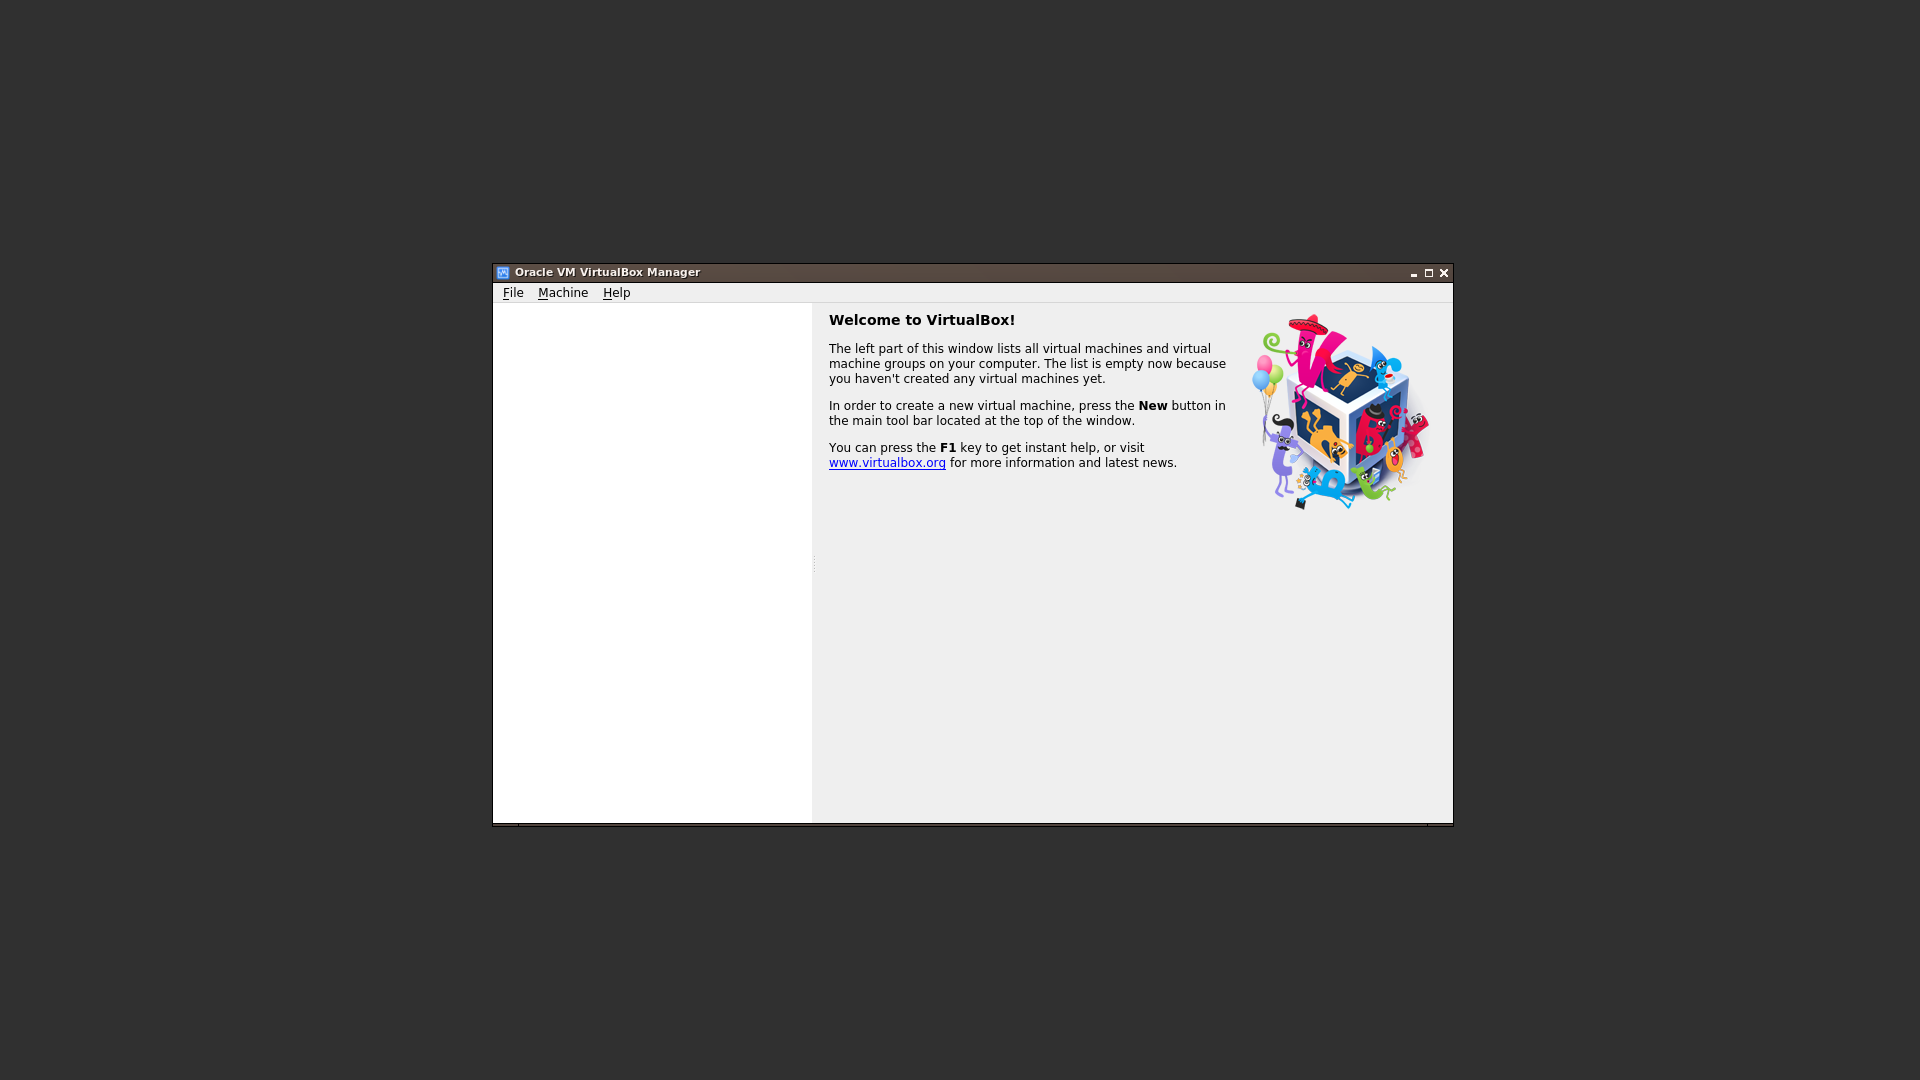
\includegraphics[width=\linewidth]{1.png}
    \caption{Запуск Vbox}
\end{figure}

\begin{figure}[H]
    \centering
    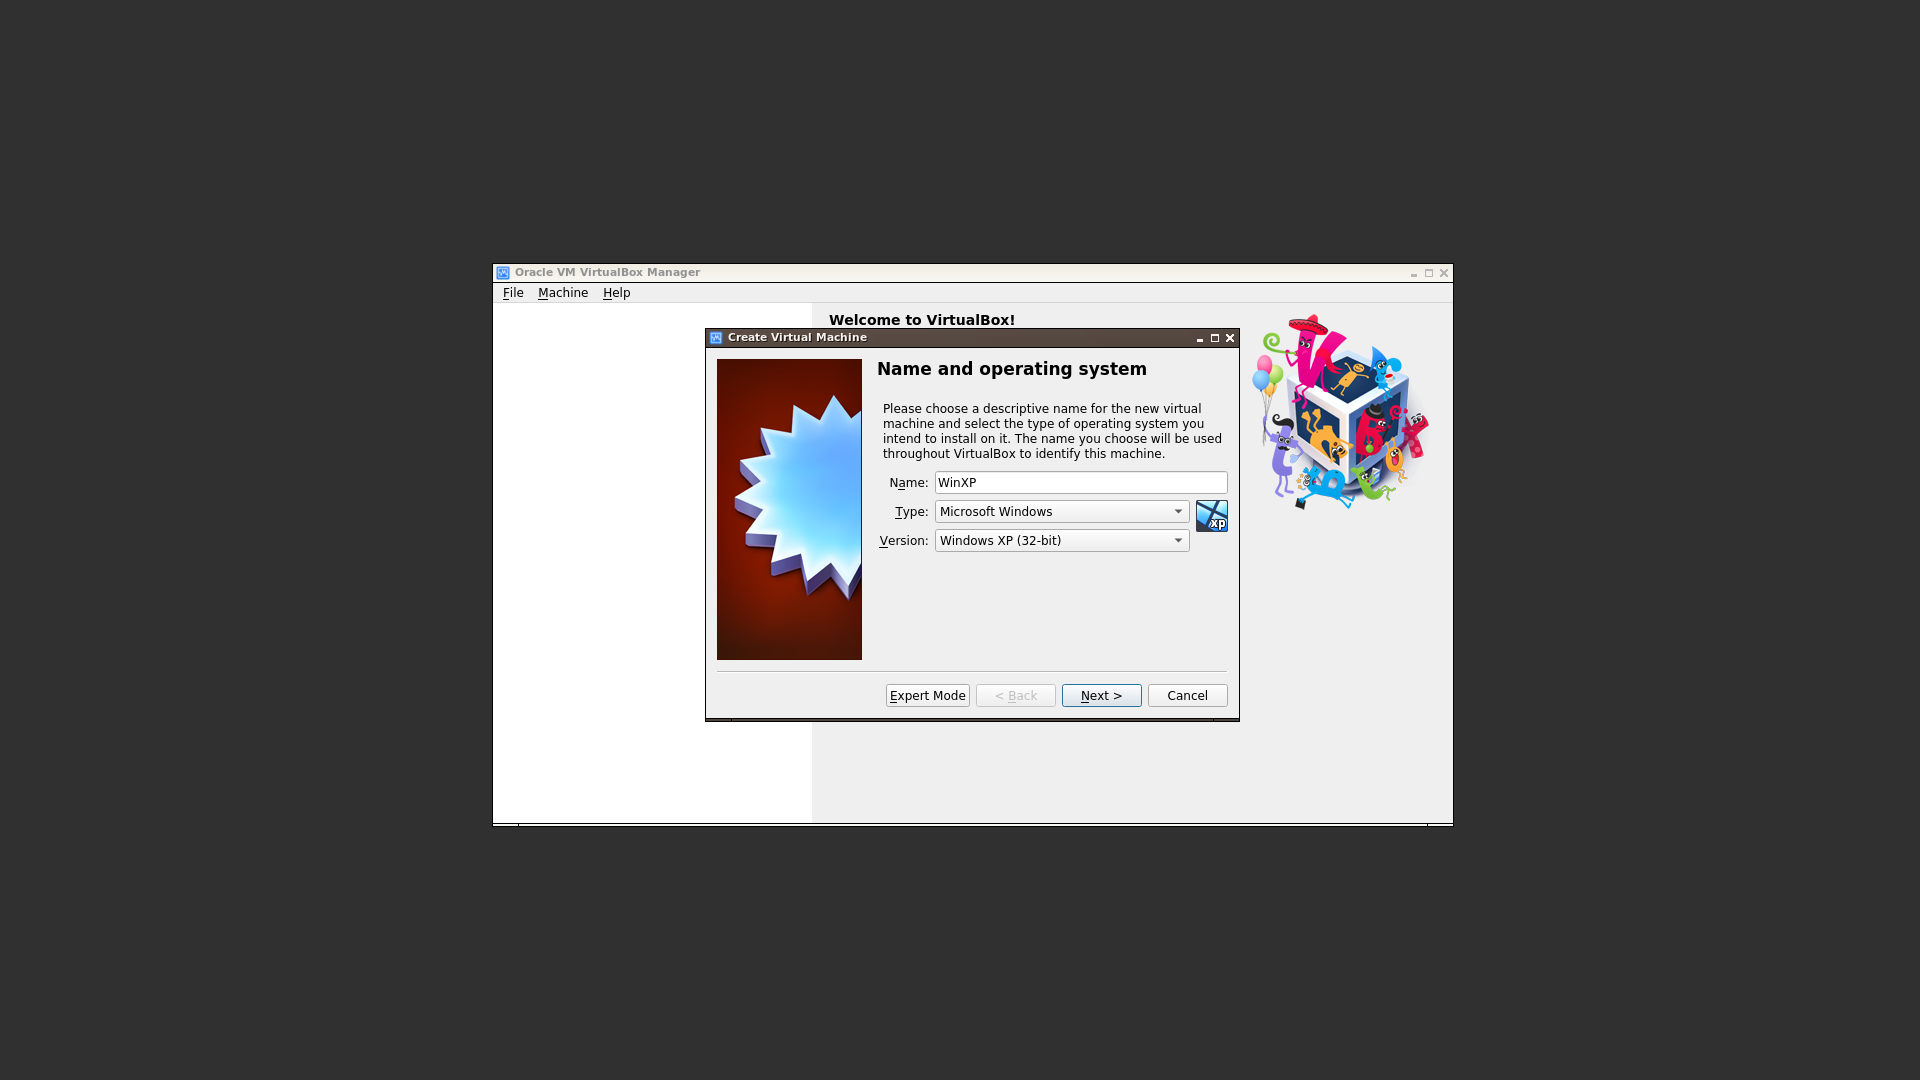
\includegraphics[width=\linewidth]{2.png}
    \caption{Выбираю название VM}
\end{figure}

\begin{figure}[H]
    \centering
    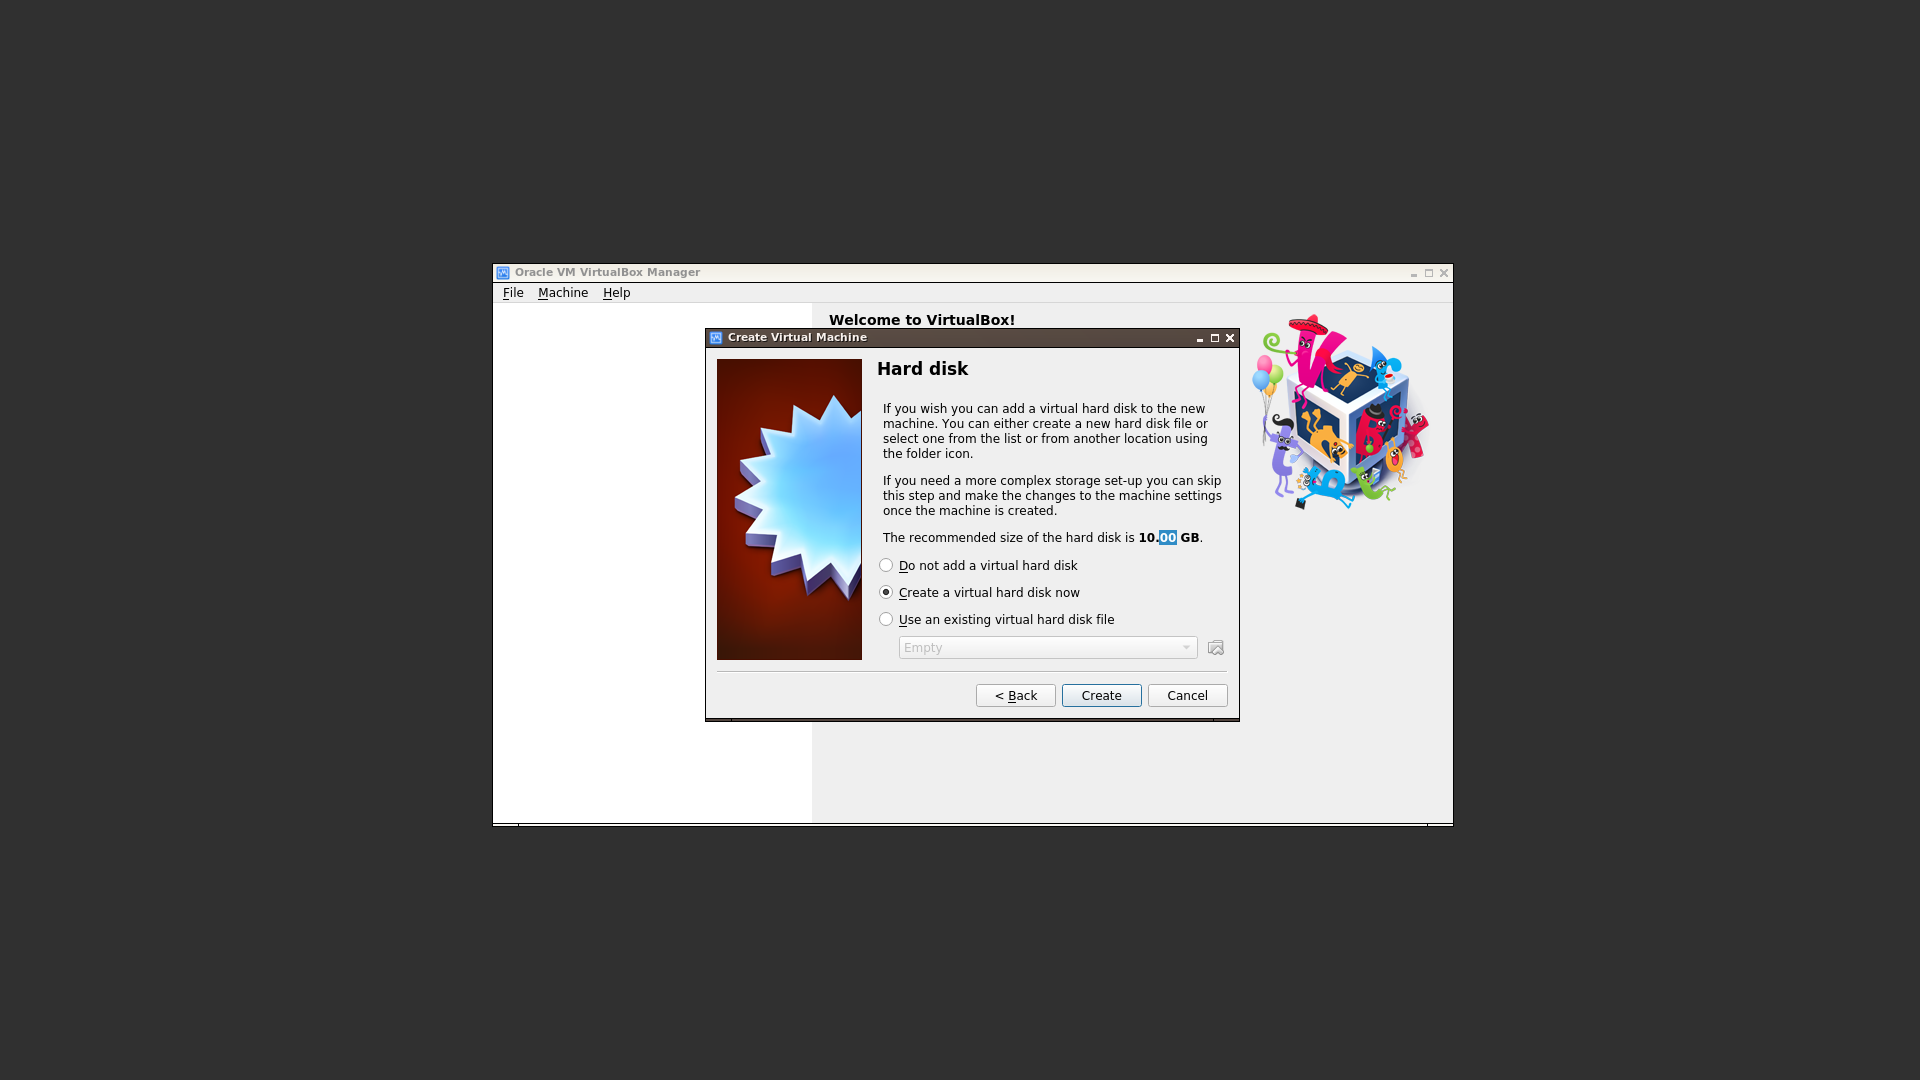
\includegraphics[width=\linewidth]{3.png}
    \caption{Создаю вирутальный жесткий диск}
\end{figure}

\begin{figure}[H]
    \centering
    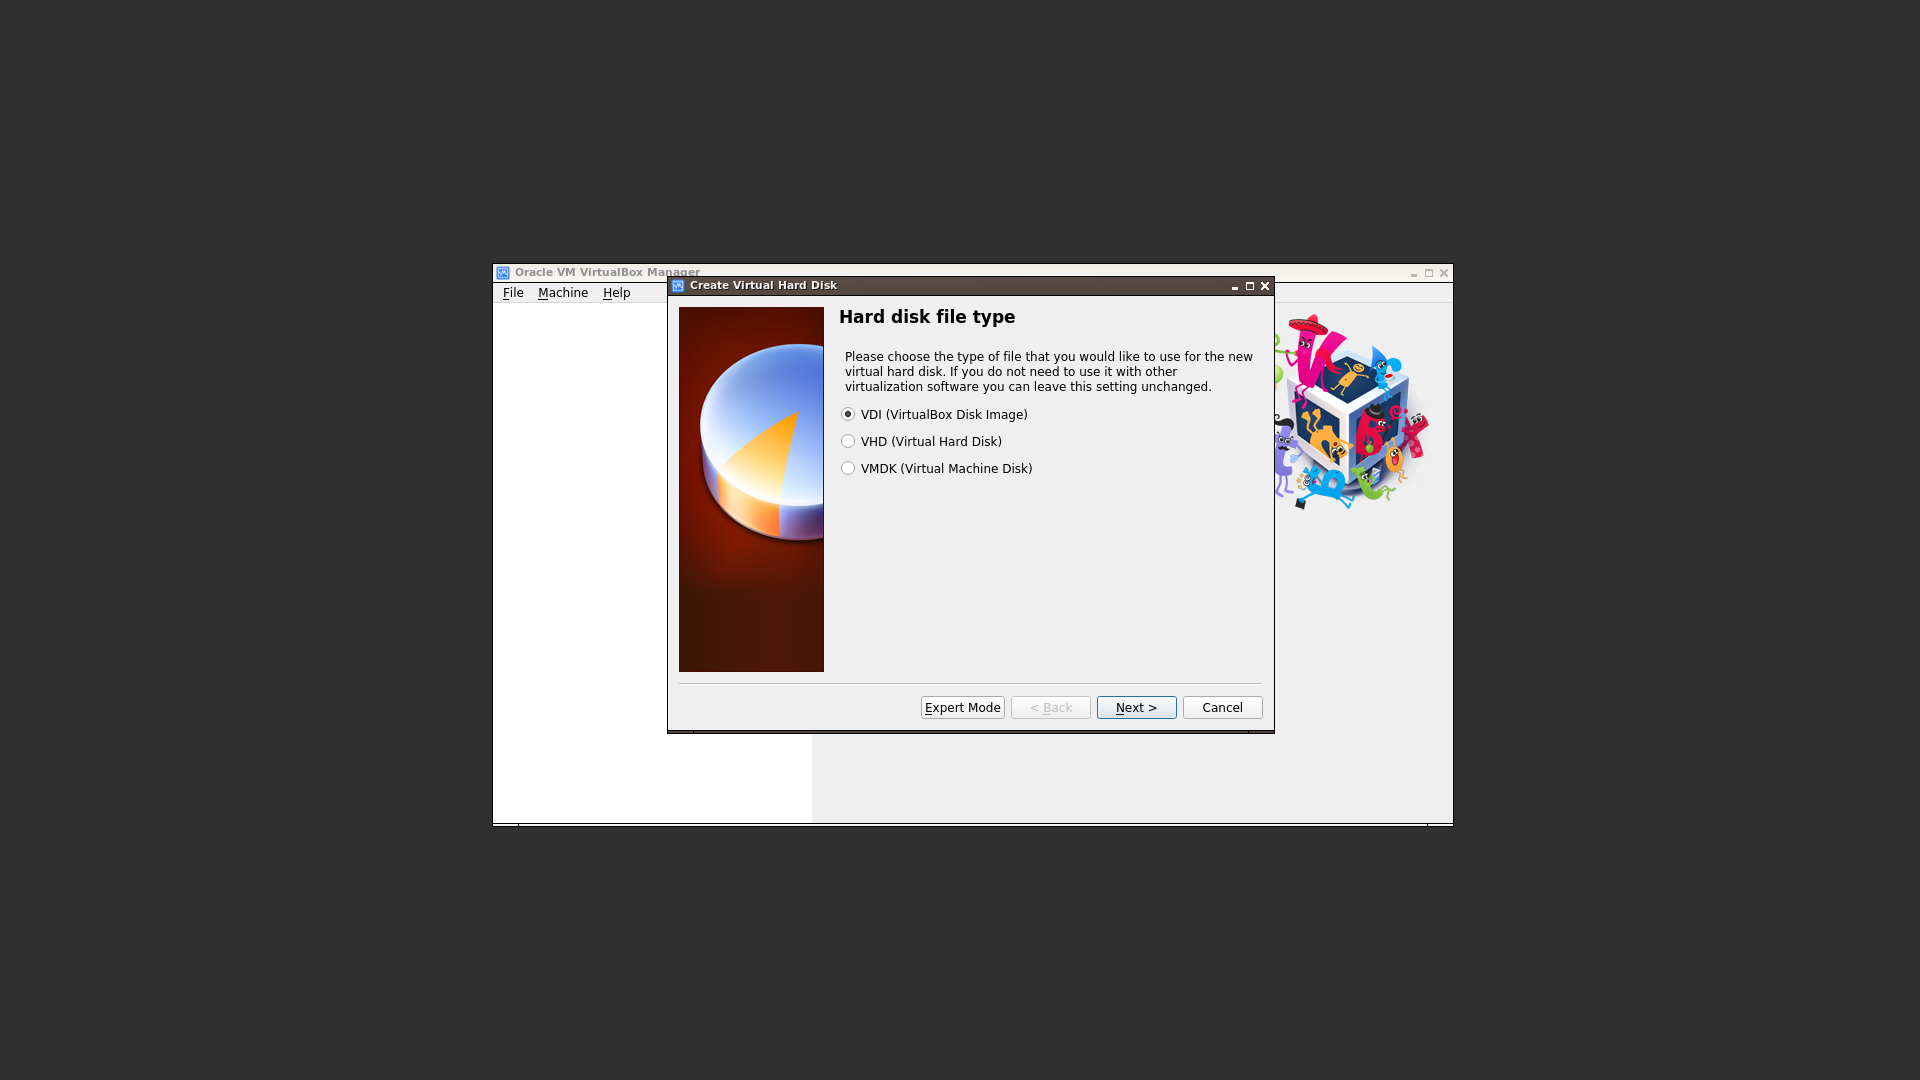
\includegraphics[width=\linewidth]{4.png}
    \caption{Выбираю тип жетского диска}
\end{figure}

\begin{figure}[H]
    \centering
    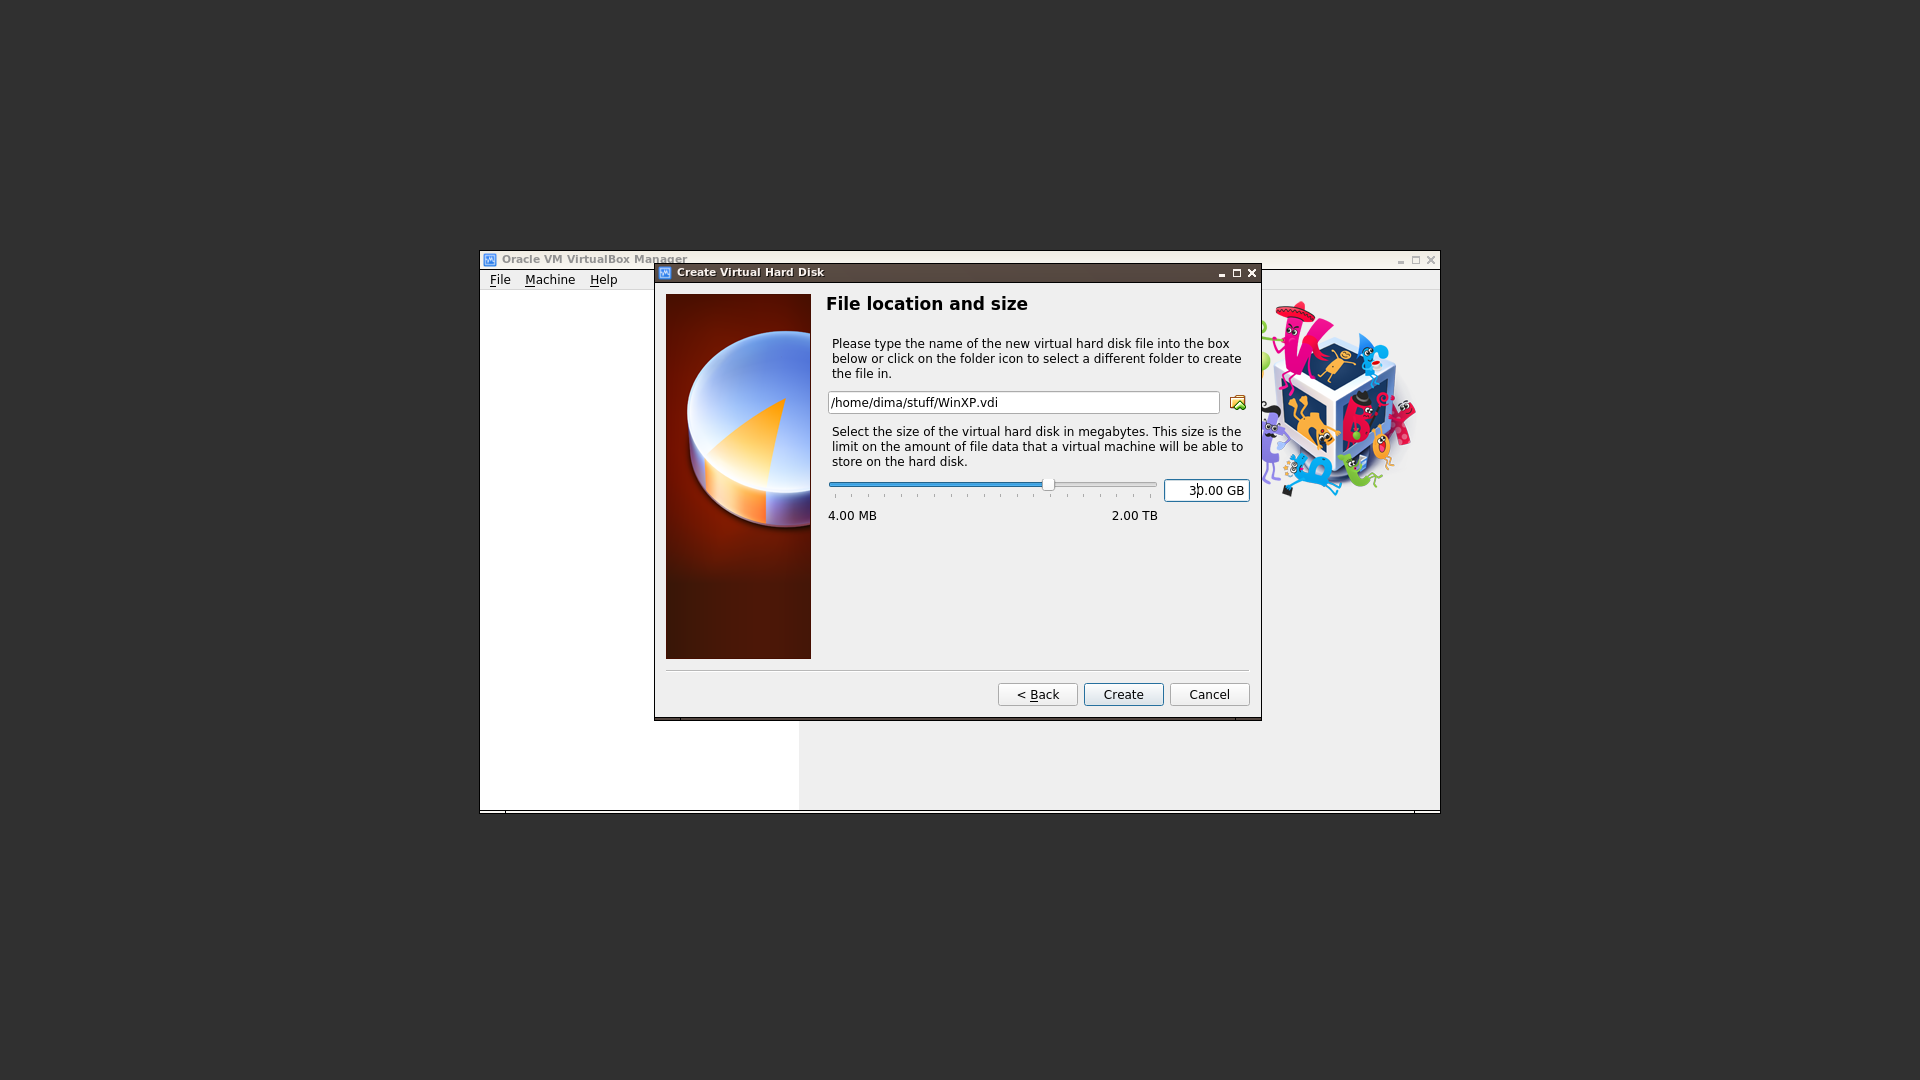
\includegraphics[width=\linewidth]{5.png}
    \caption{Выбираю 30Gb}
\end{figure}

\begin{figure}[H]
    \centering
    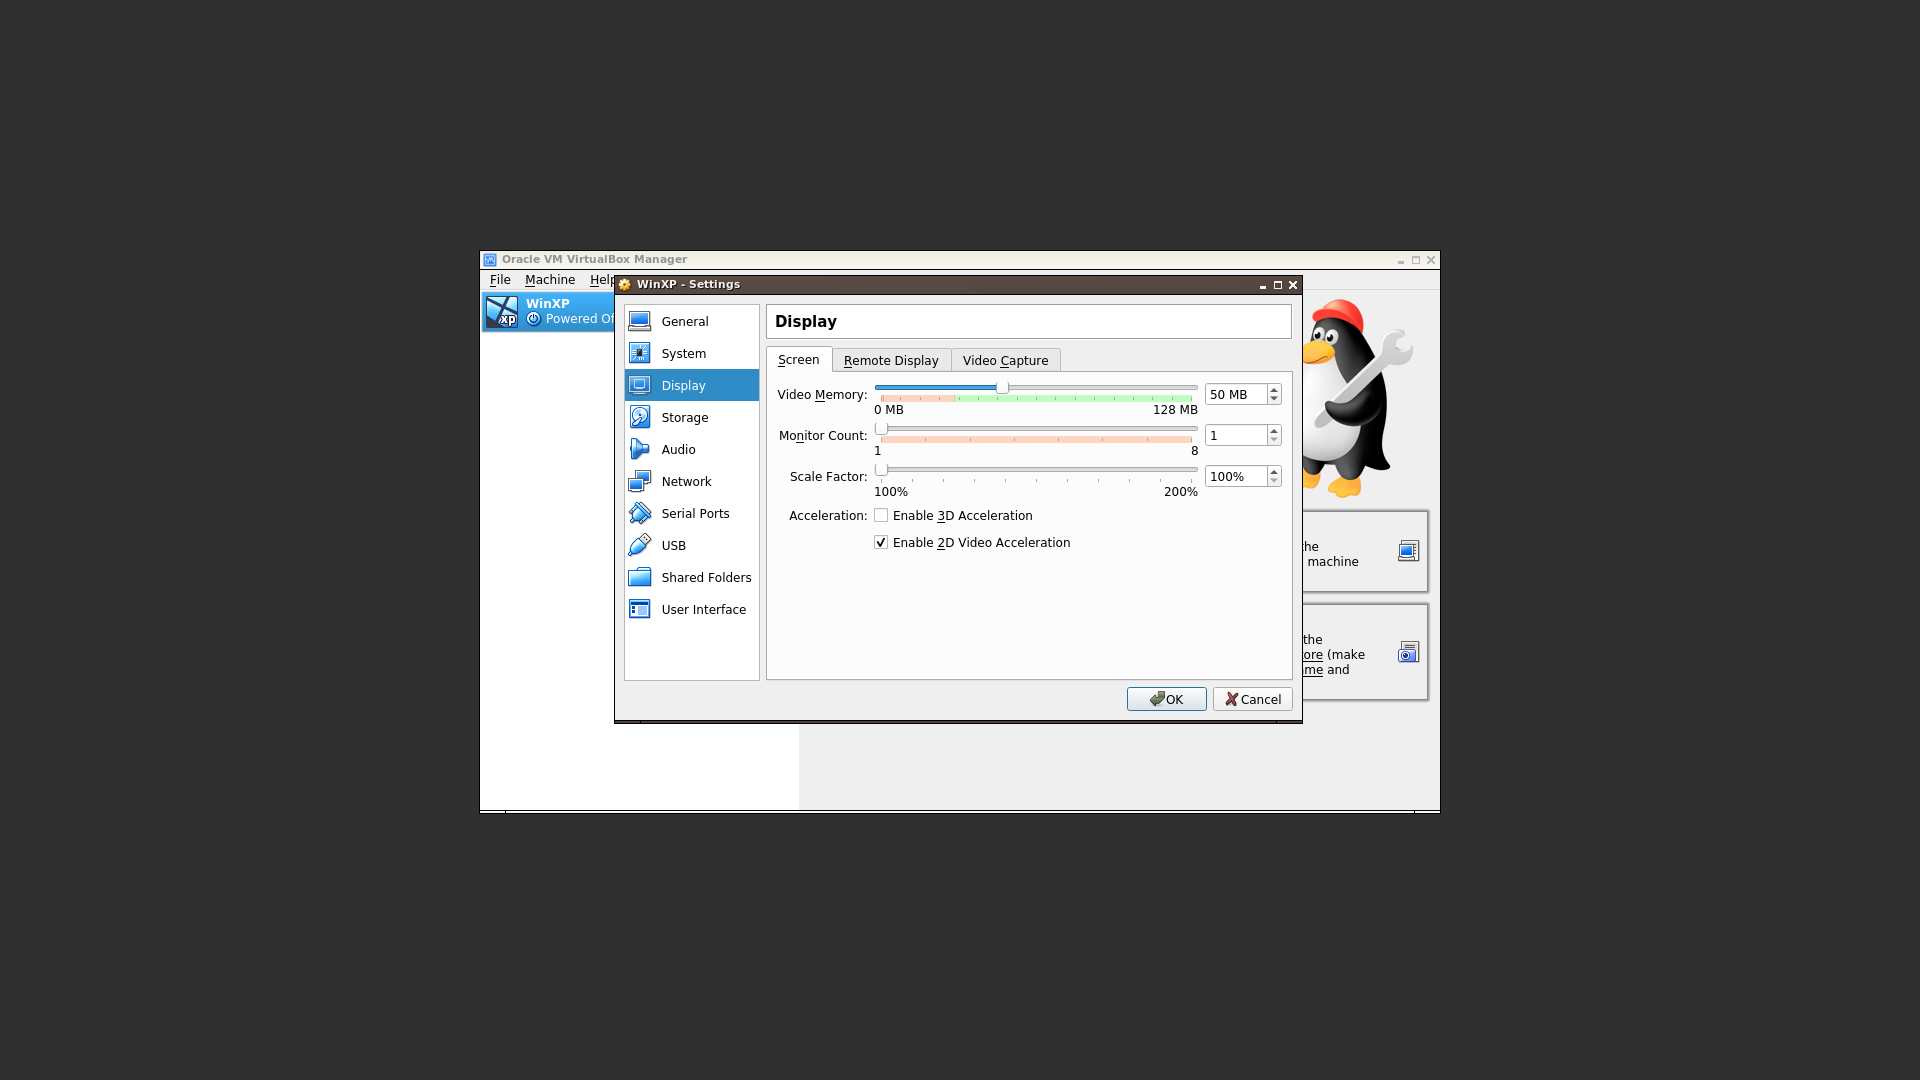
\includegraphics[width=\linewidth]{7.png}
    \caption{Включаю 2D ускорени}
\end{figure}

\begin{figure}[H]
    \centering
    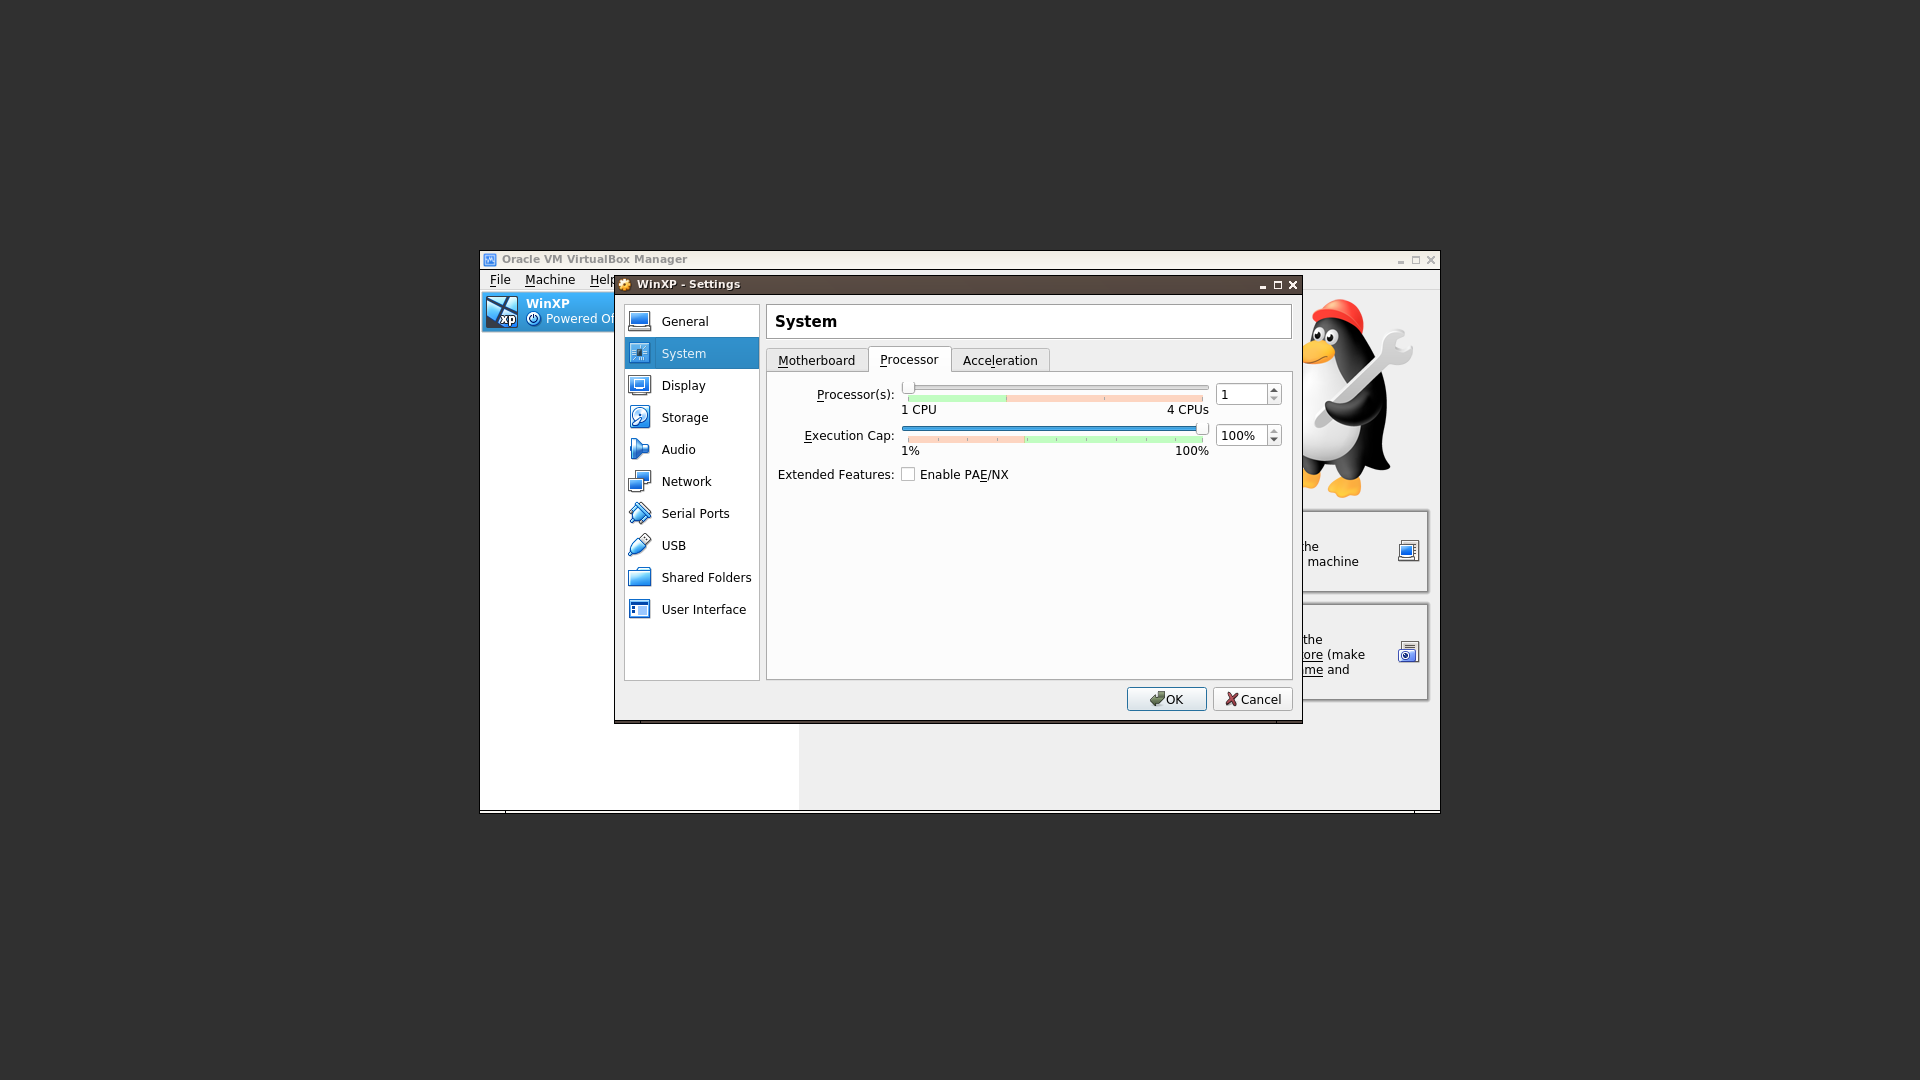
\includegraphics[width=\linewidth]{8.png}
    \caption{Предел загрузки CPU 100\%}
\end{figure}

\begin{figure}[H]
    \centering
    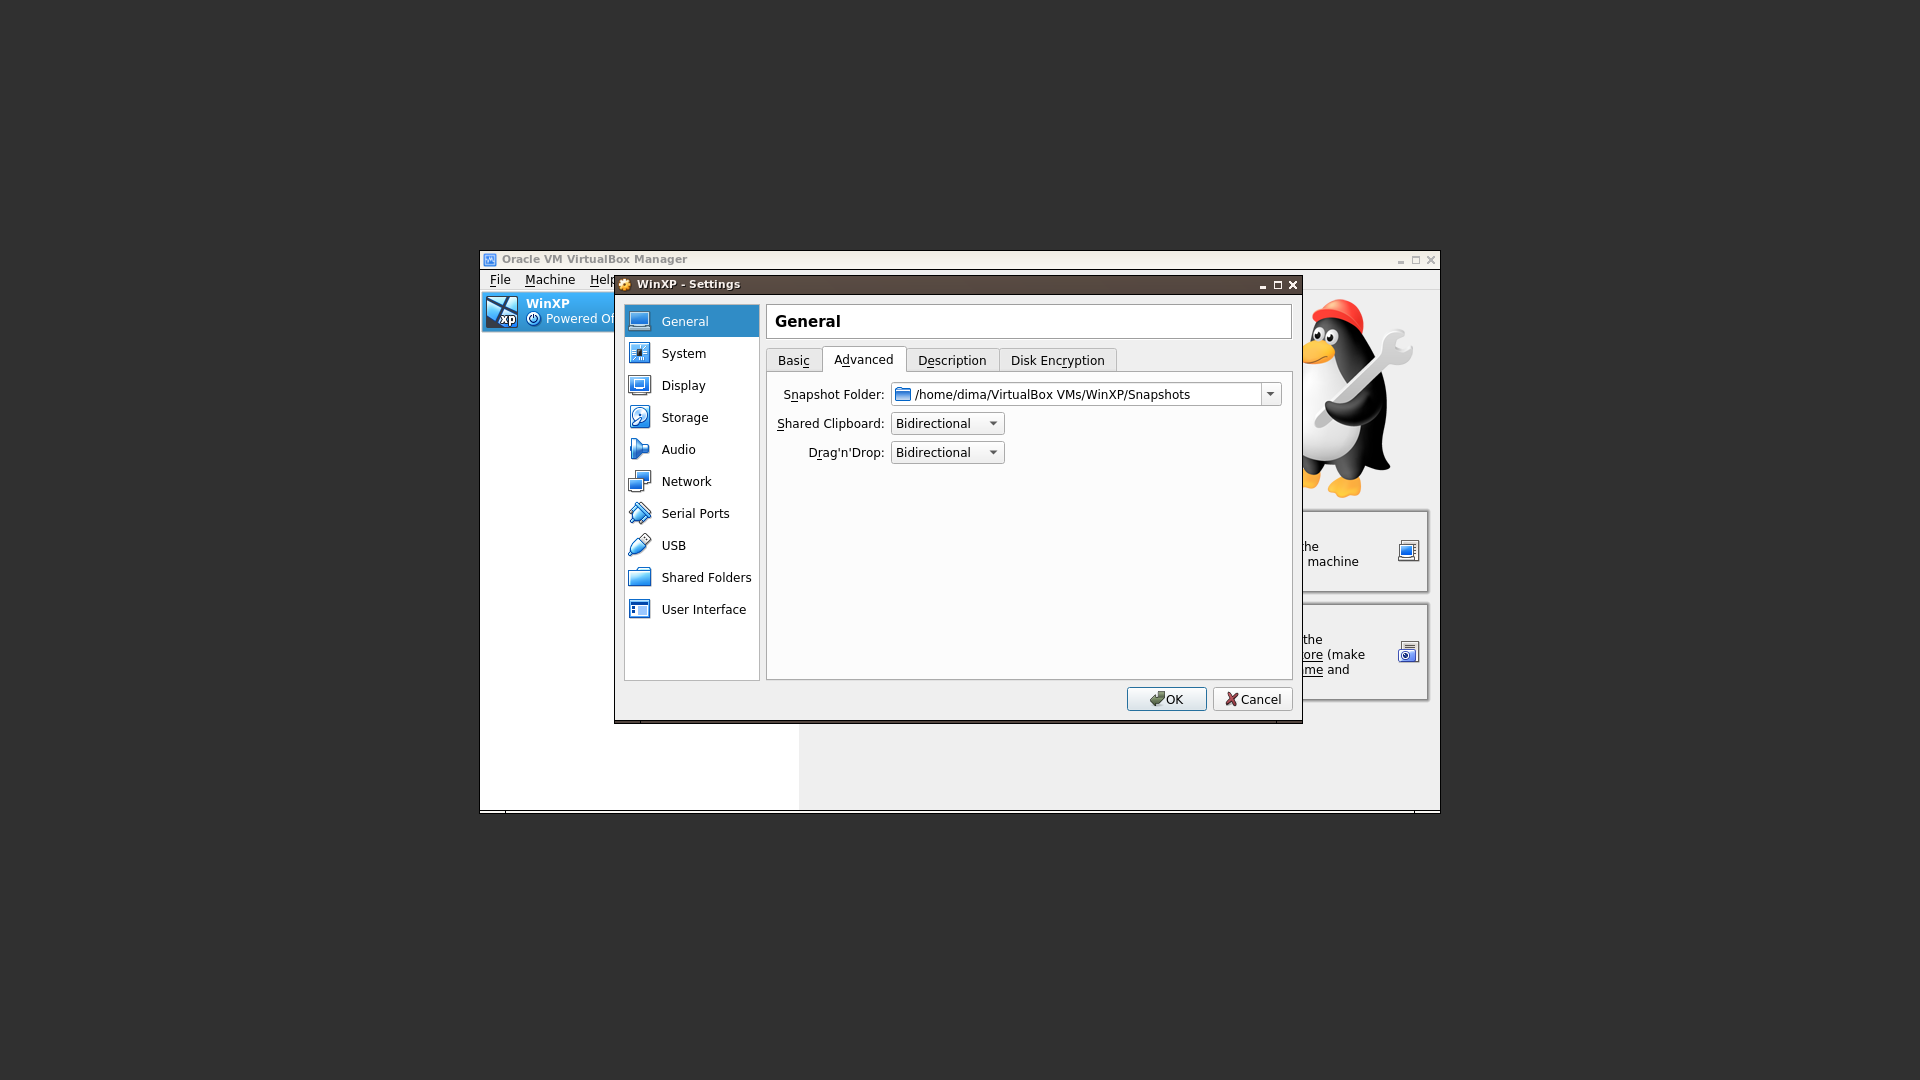
\includegraphics[width=\linewidth]{9.png}
    \caption{Включаю drag and drop and clipboard}
\end{figure}

\begin{figure}[H]
    \centering
    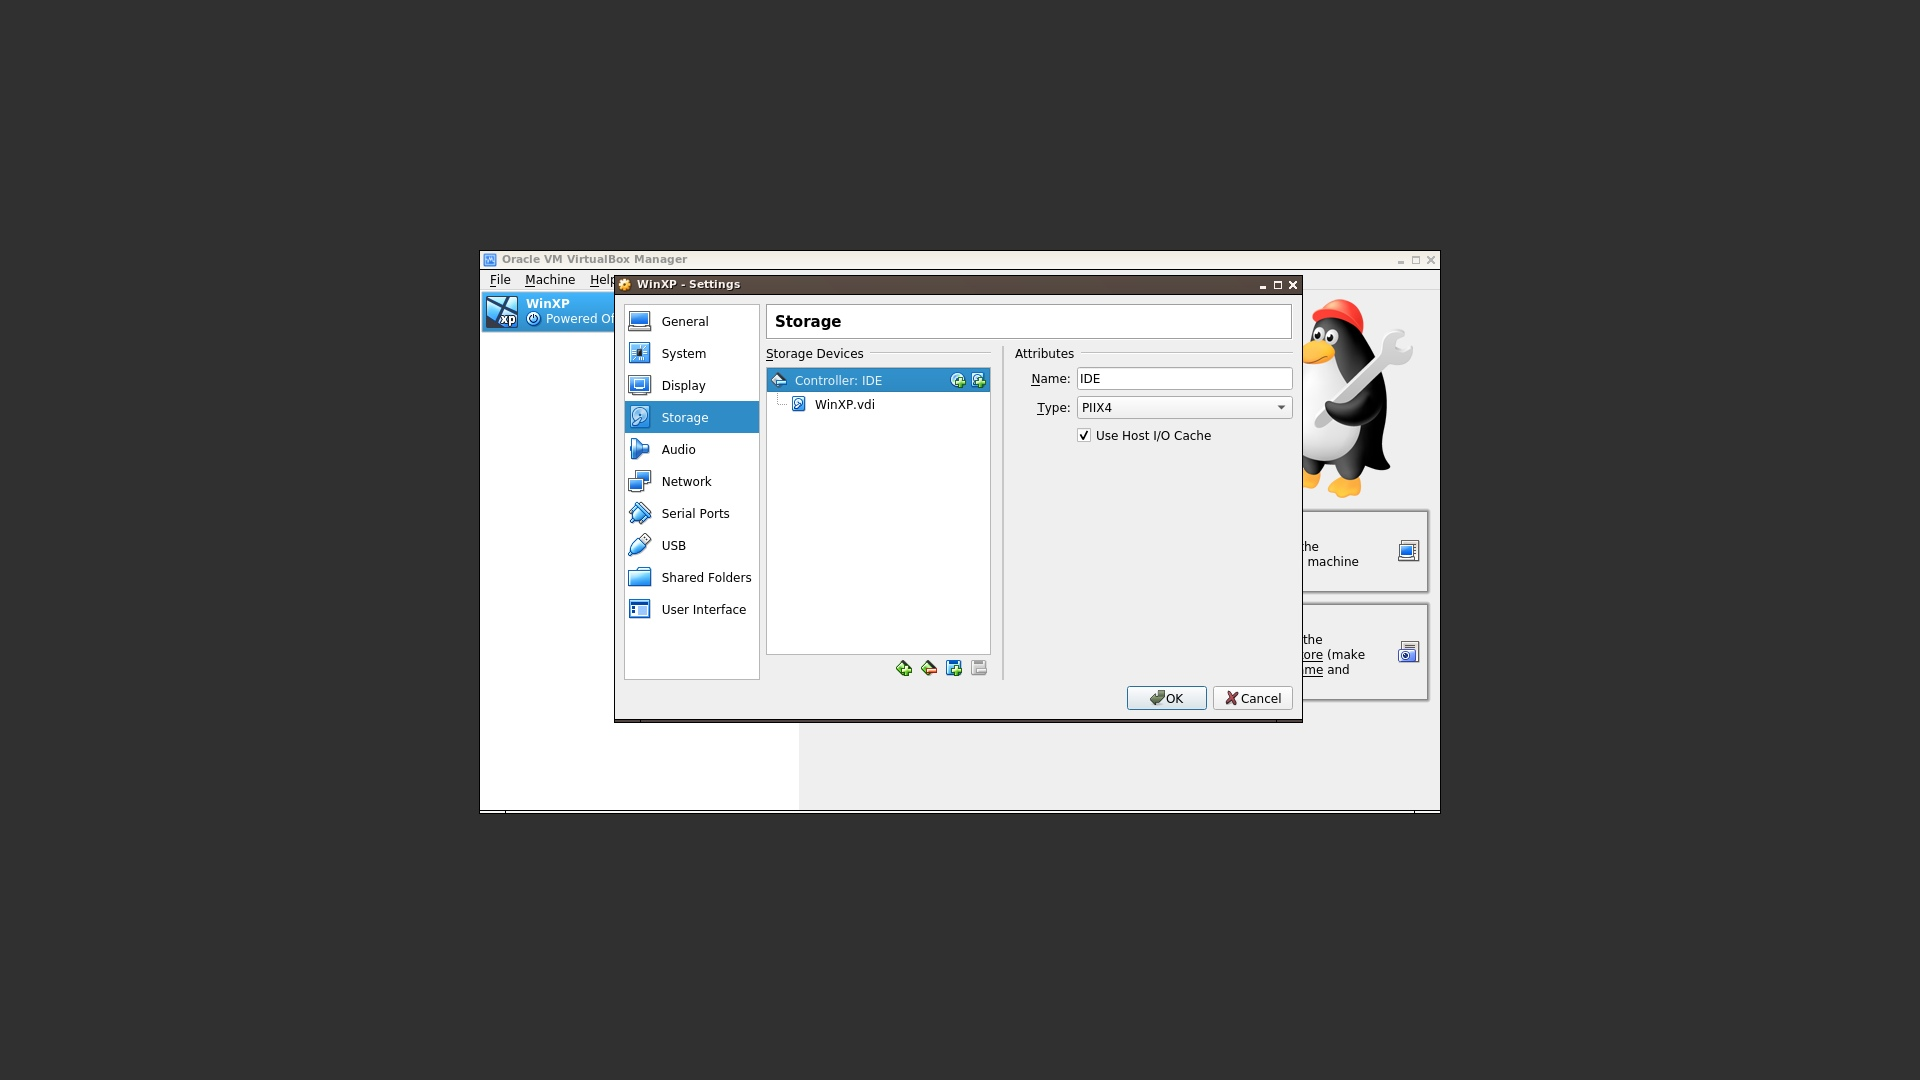
\includegraphics[width=\linewidth]{10-1.png}
    \caption{Включаю кэширование I/O}
\end{figure}

\subsection{Установка ОС}
\begin{figure}[H]
    \centering
    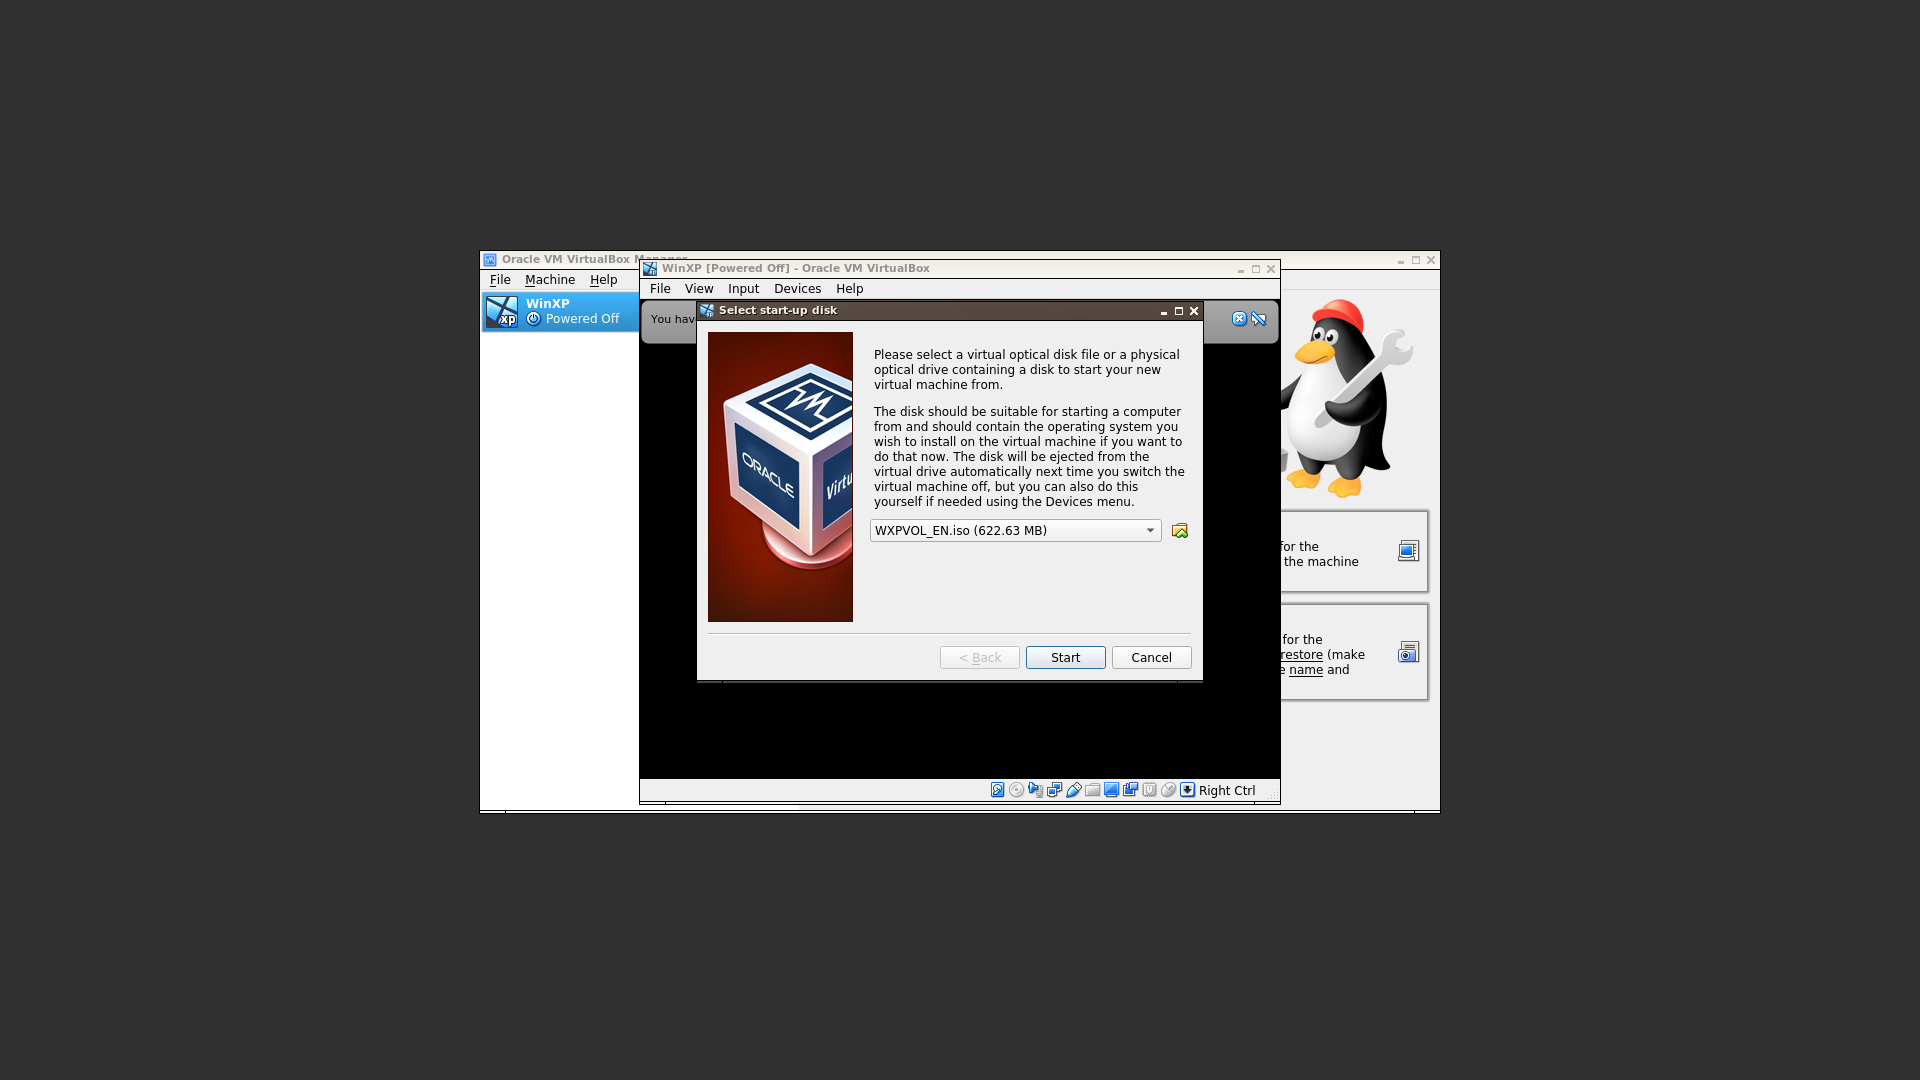
\includegraphics[width=\linewidth]{13.png}
    \caption{Выбираю образ ОС}
\end{figure}

\begin{figure}[H]
    \centering
    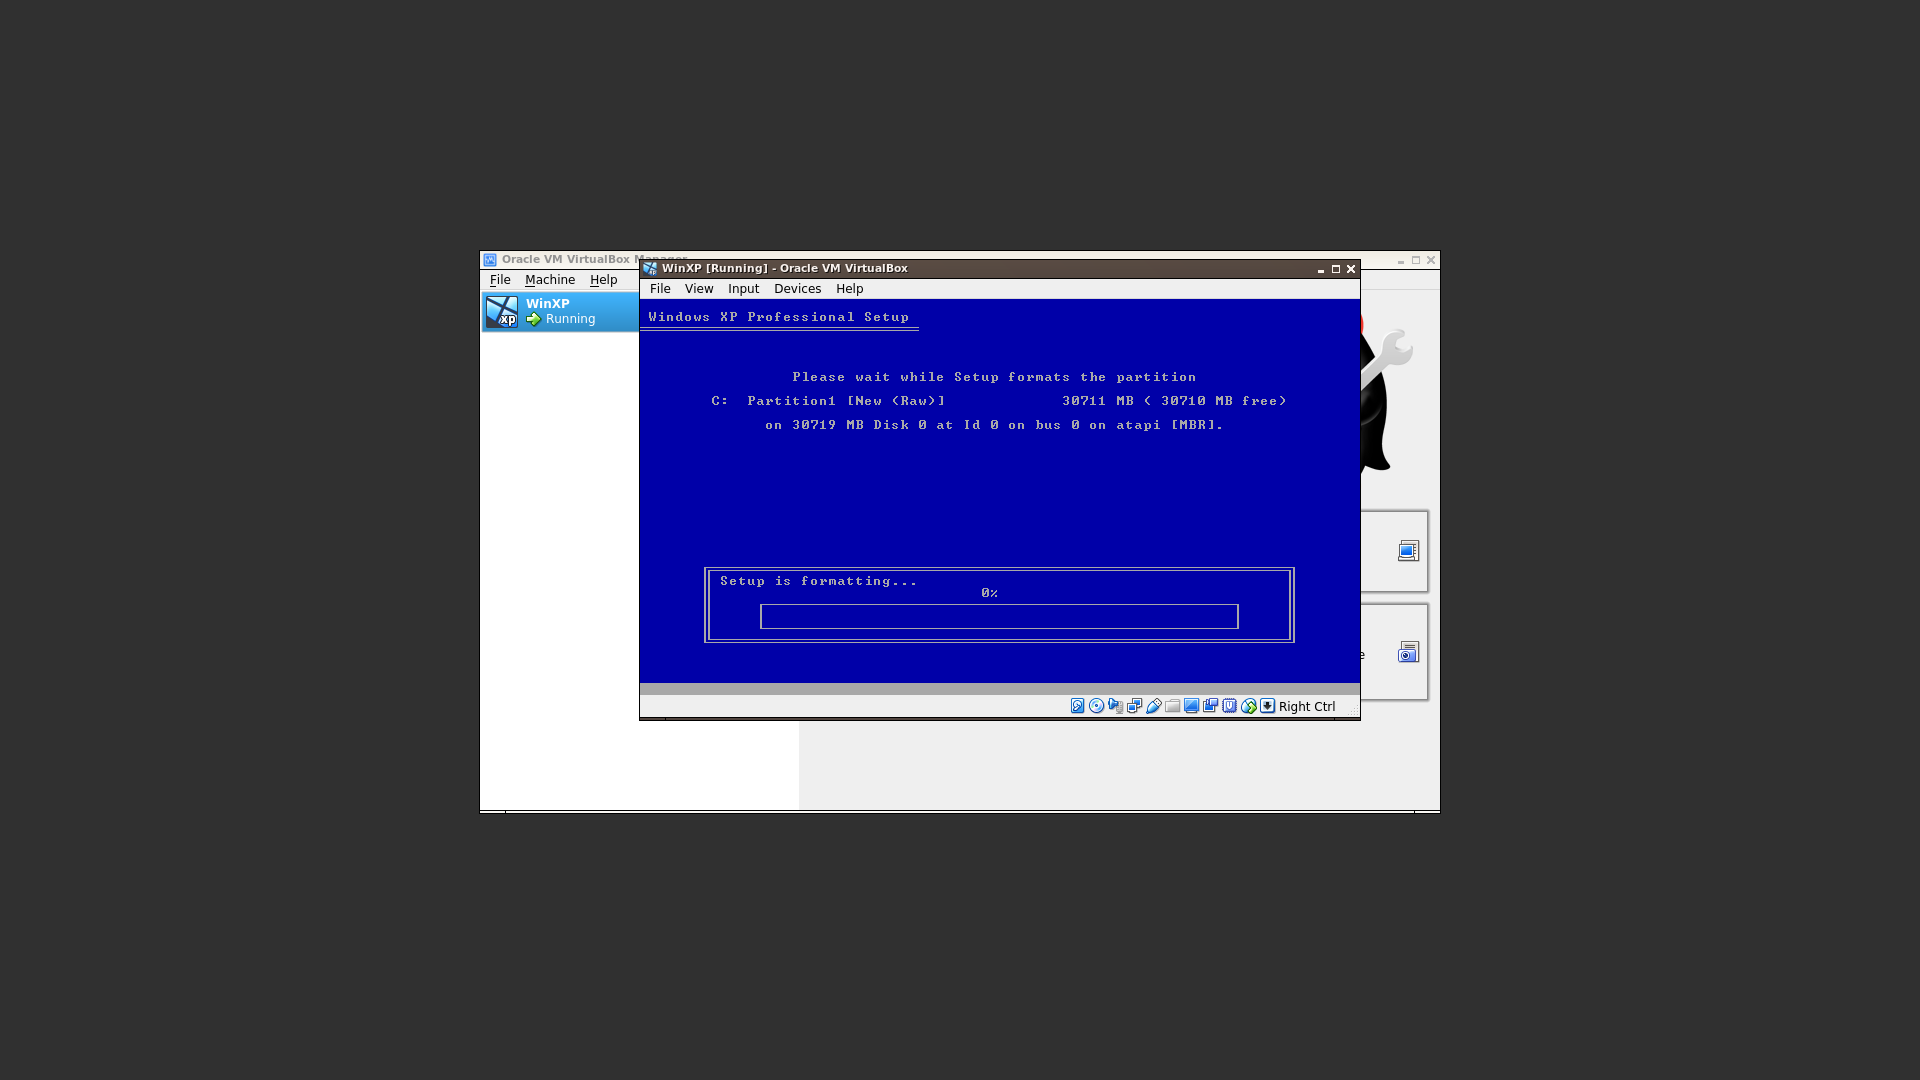
\includegraphics[width=\linewidth]{15.png}
    \caption{Создаю раздела под диск C:}
\end{figure}

\begin{figure}[H]
    \centering
    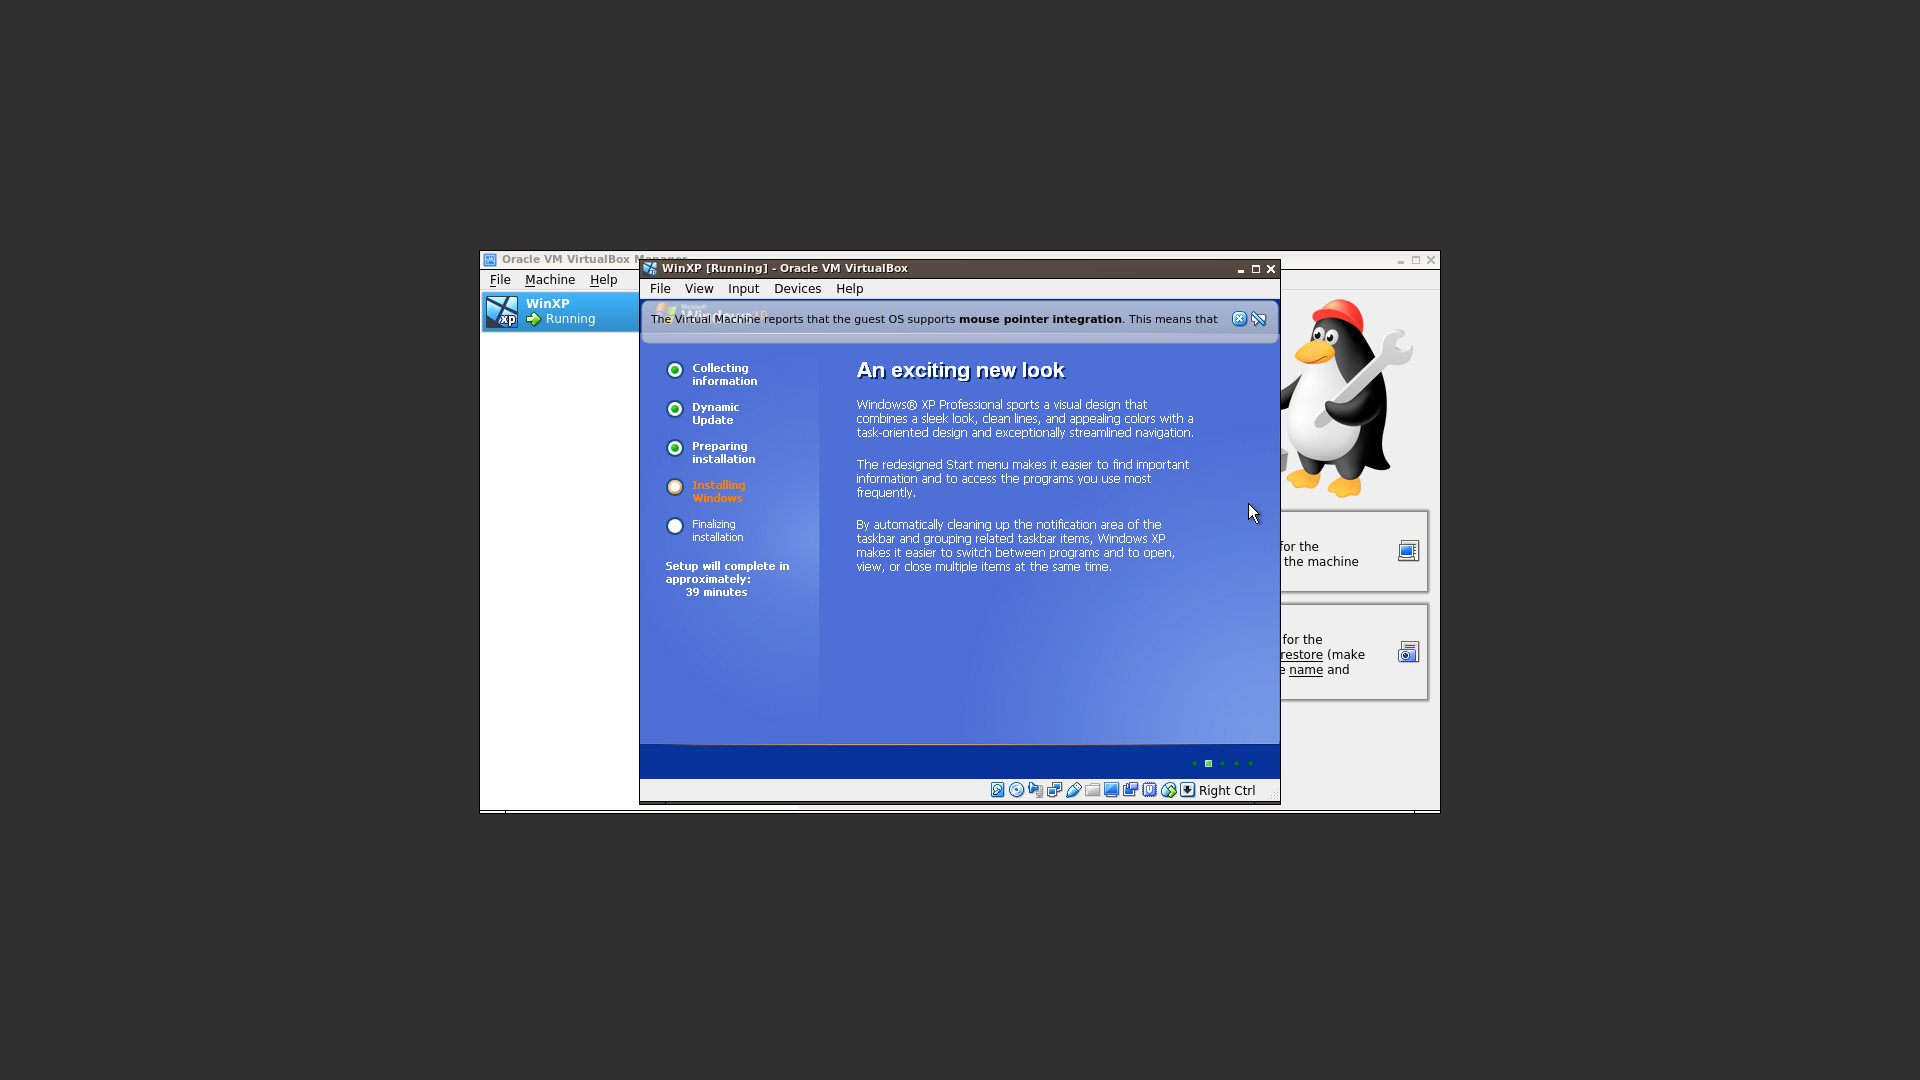
\includegraphics[width=\linewidth]{16.png}
    \caption{Перезагрузилось в графический установщик}
\end{figure}

\begin{figure}[H]
    \centering
    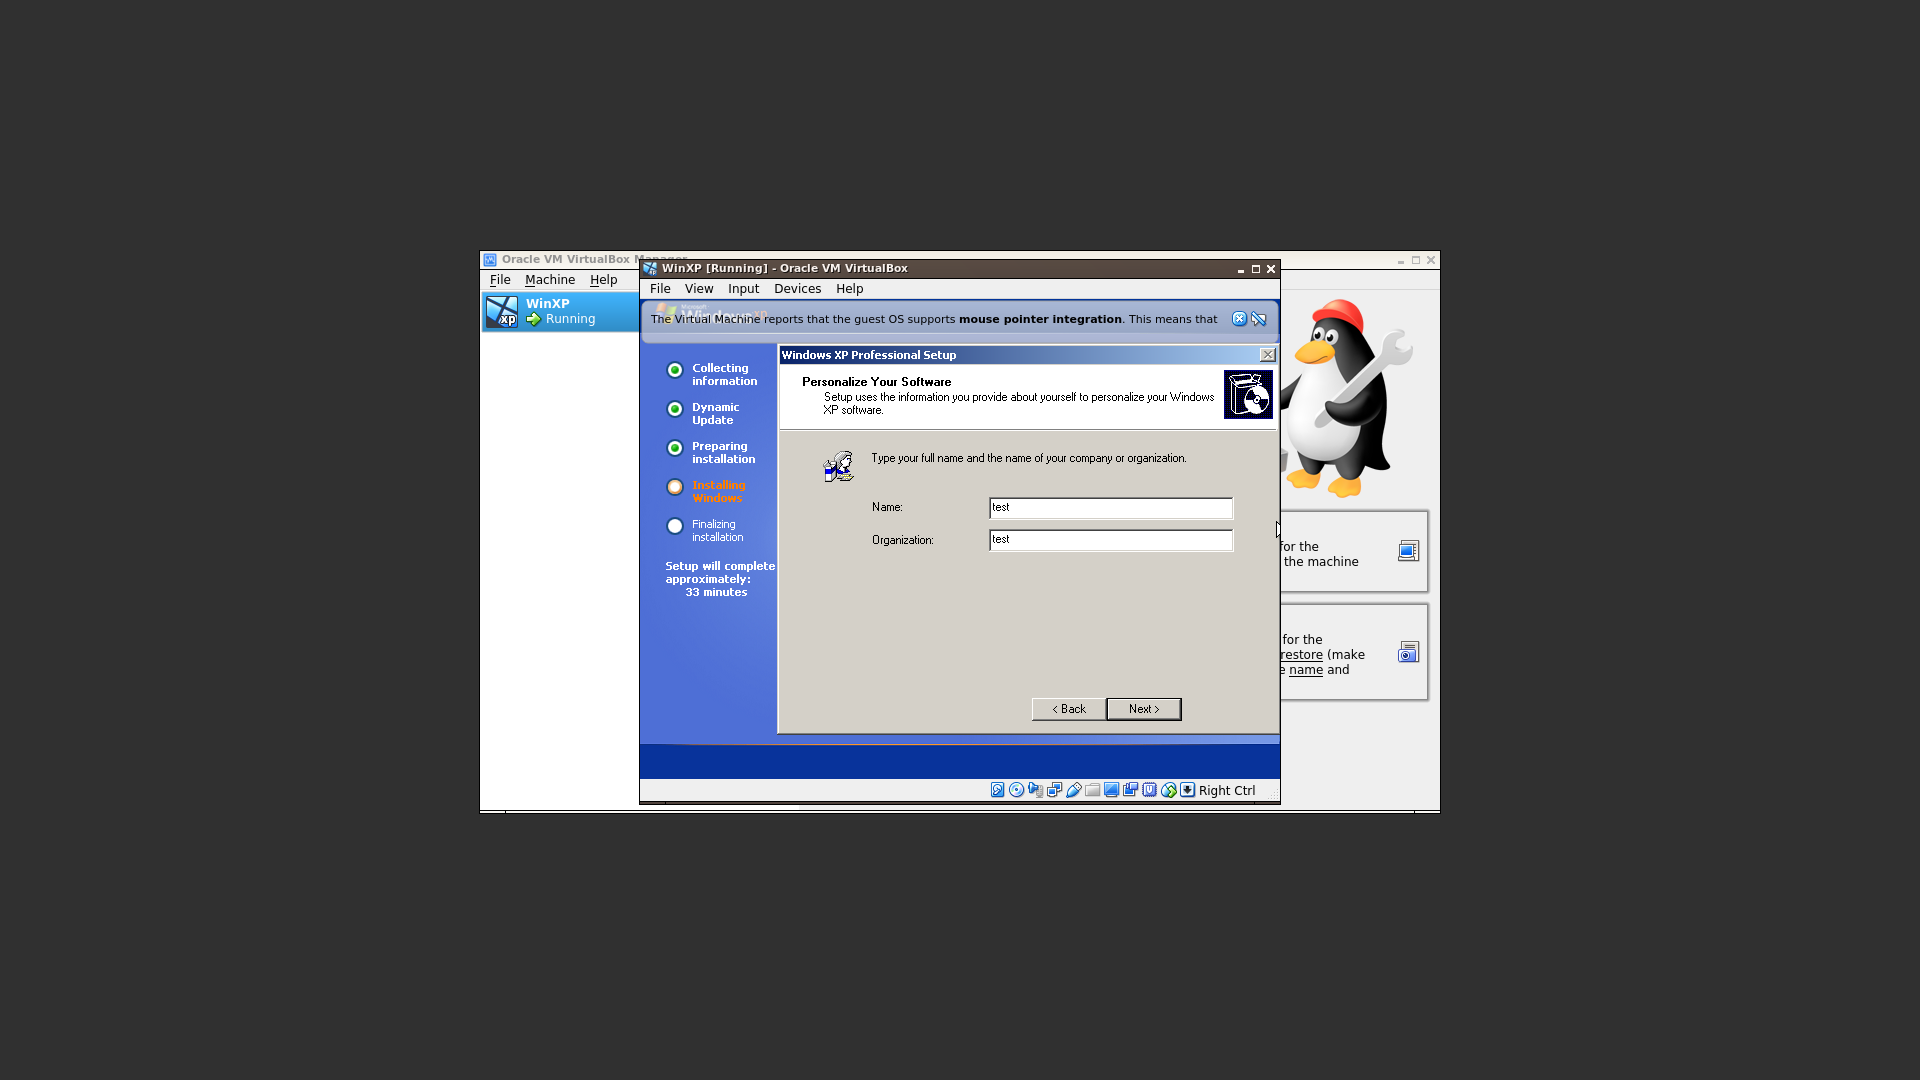
\includegraphics[width=\linewidth]{18.png}
\end{figure}    

\begin{figure}[H]
    \centering
    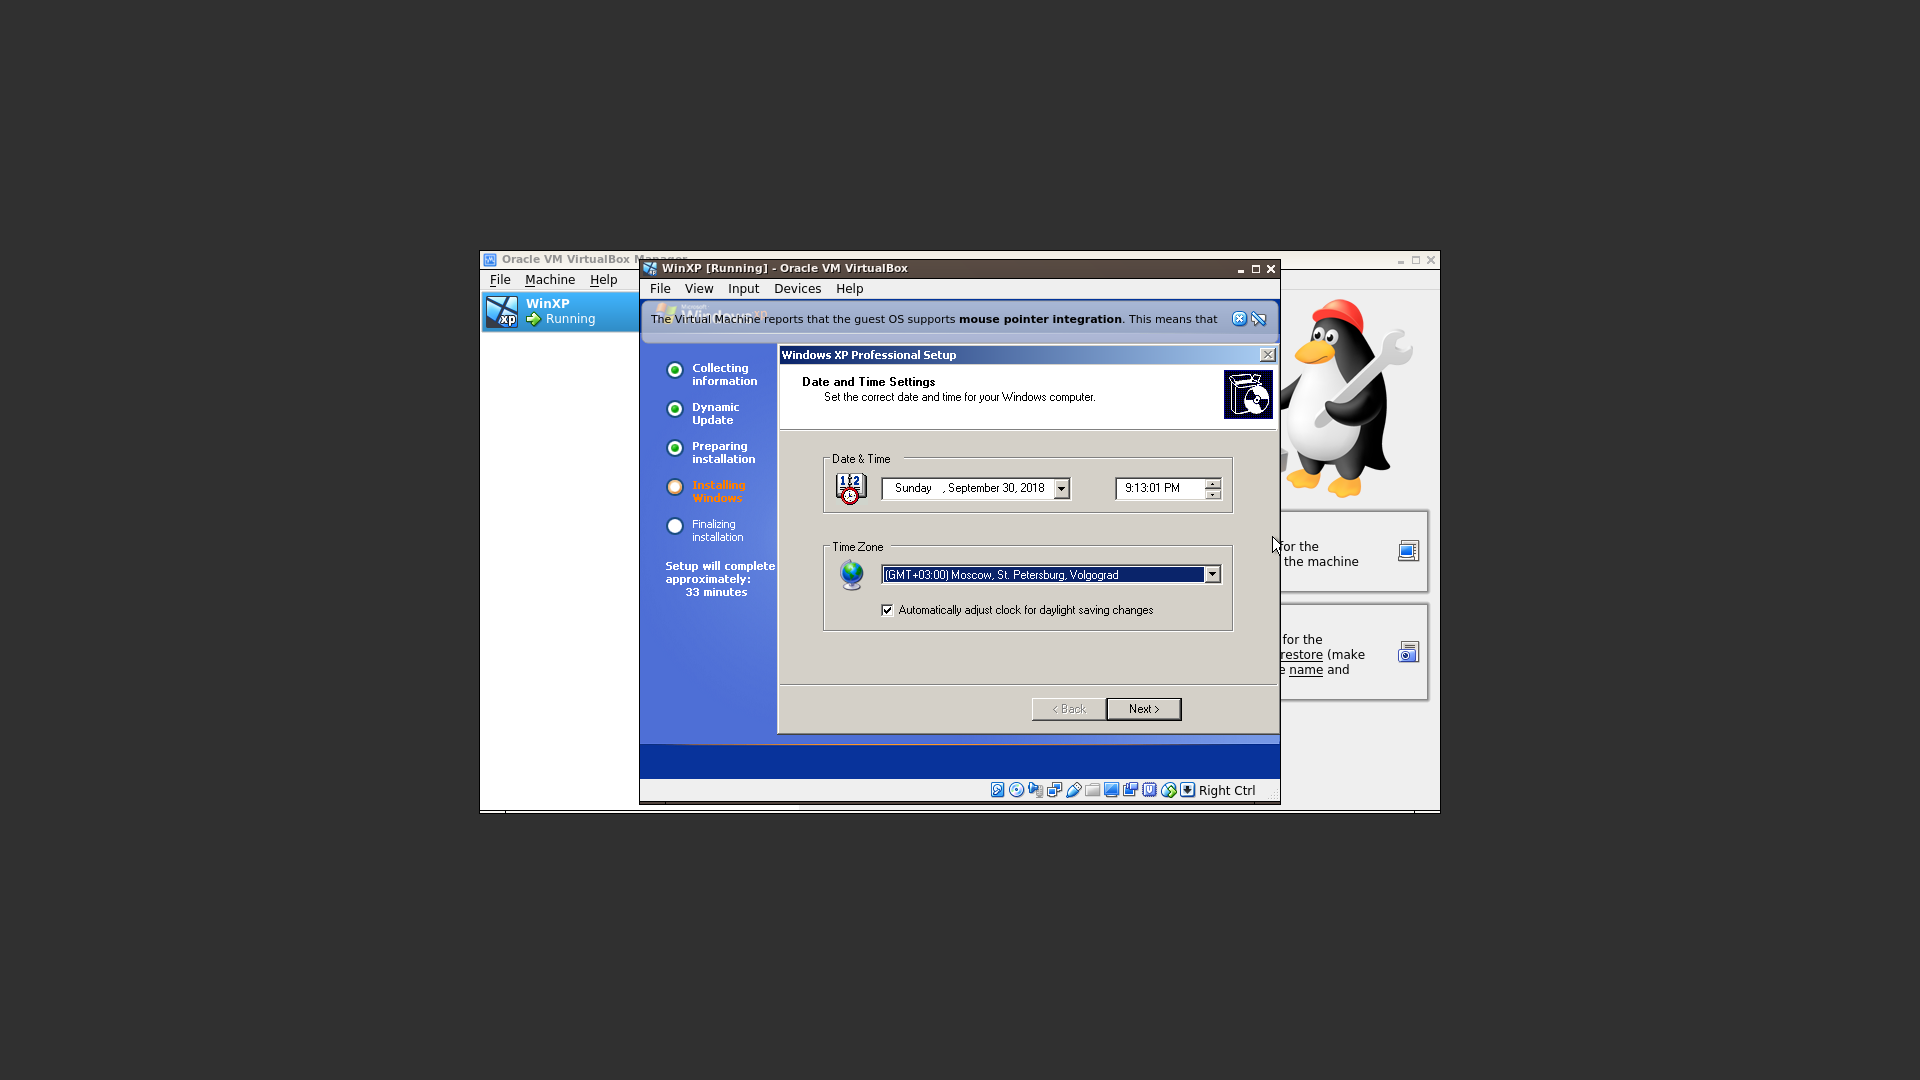
\includegraphics[width=\linewidth]{19.png}
    \caption{Время}
\end{figure}

\begin{figure}[H]
    \centering
    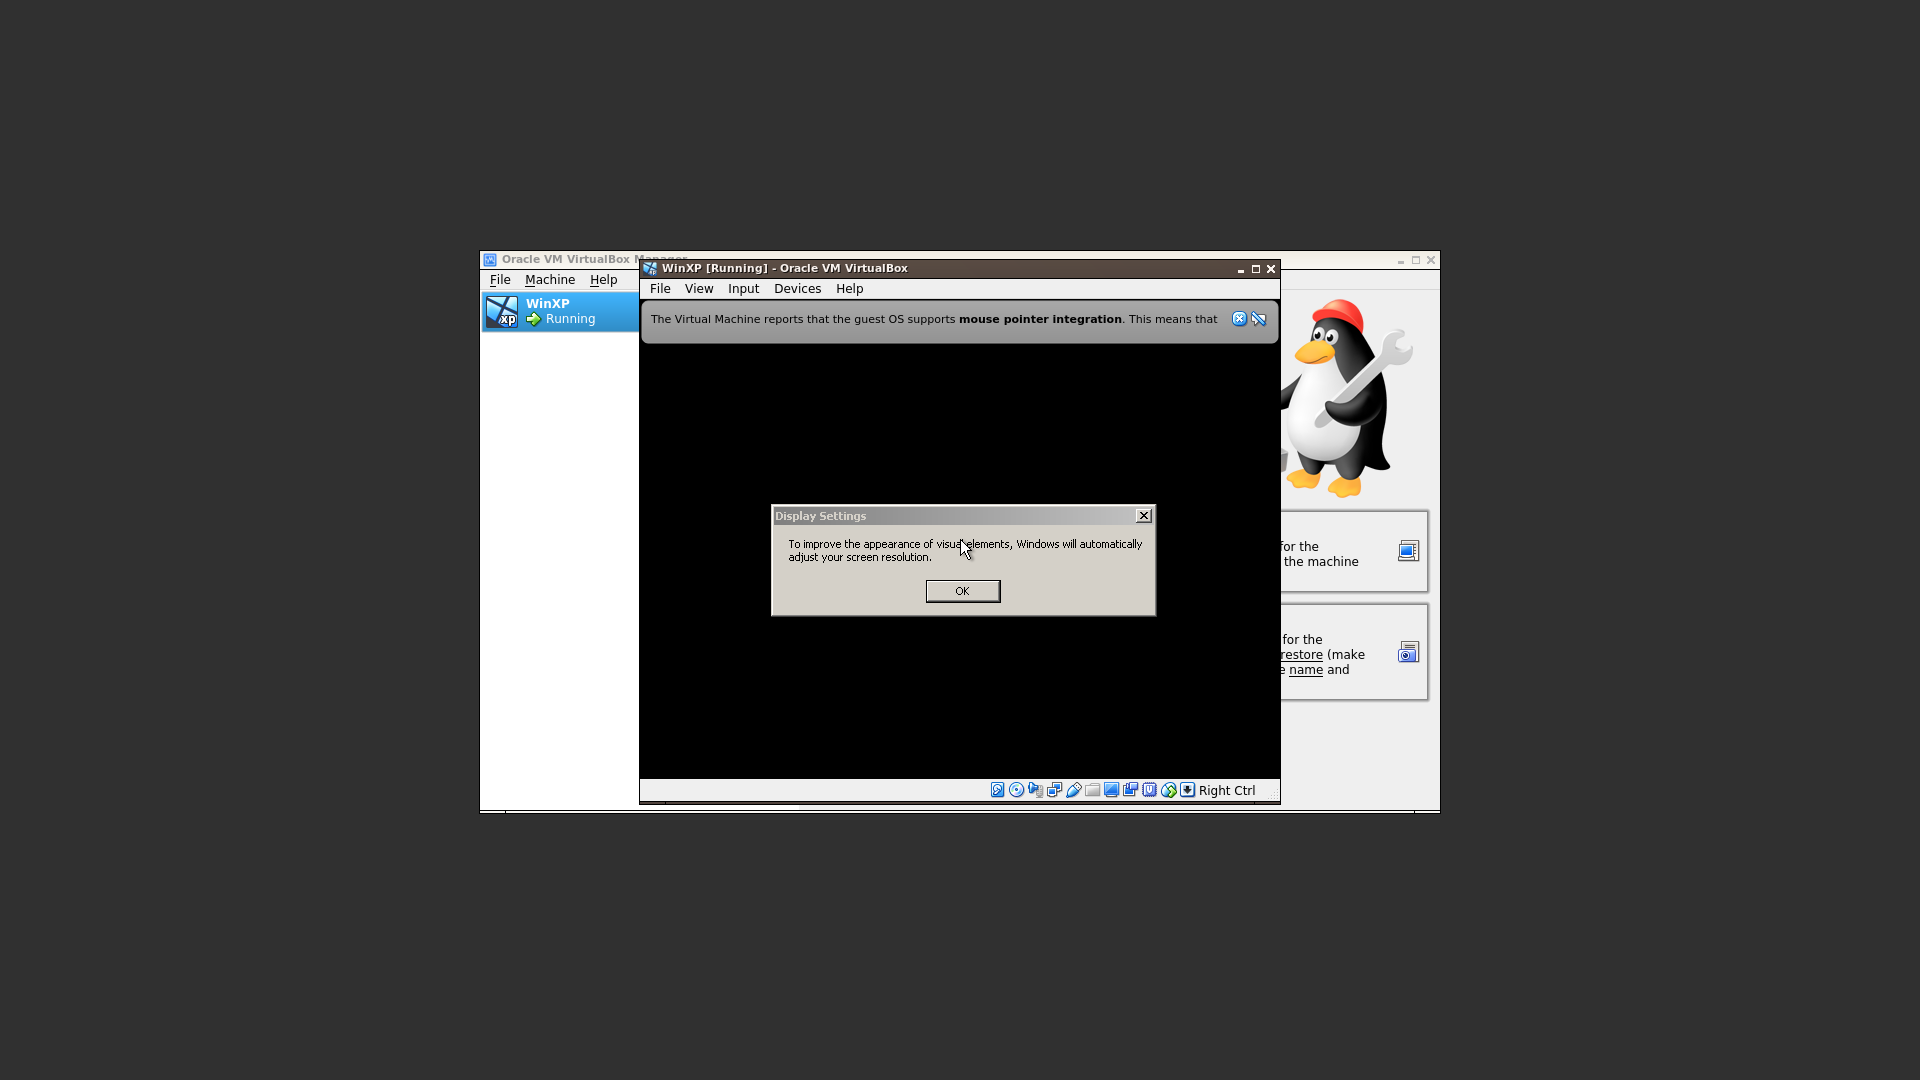
\includegraphics[width=\linewidth]{20.png}
    \caption{Предлагают переключитсья в 1024x768}
\end{figure}    

\begin{figure}[H]
    \centering
    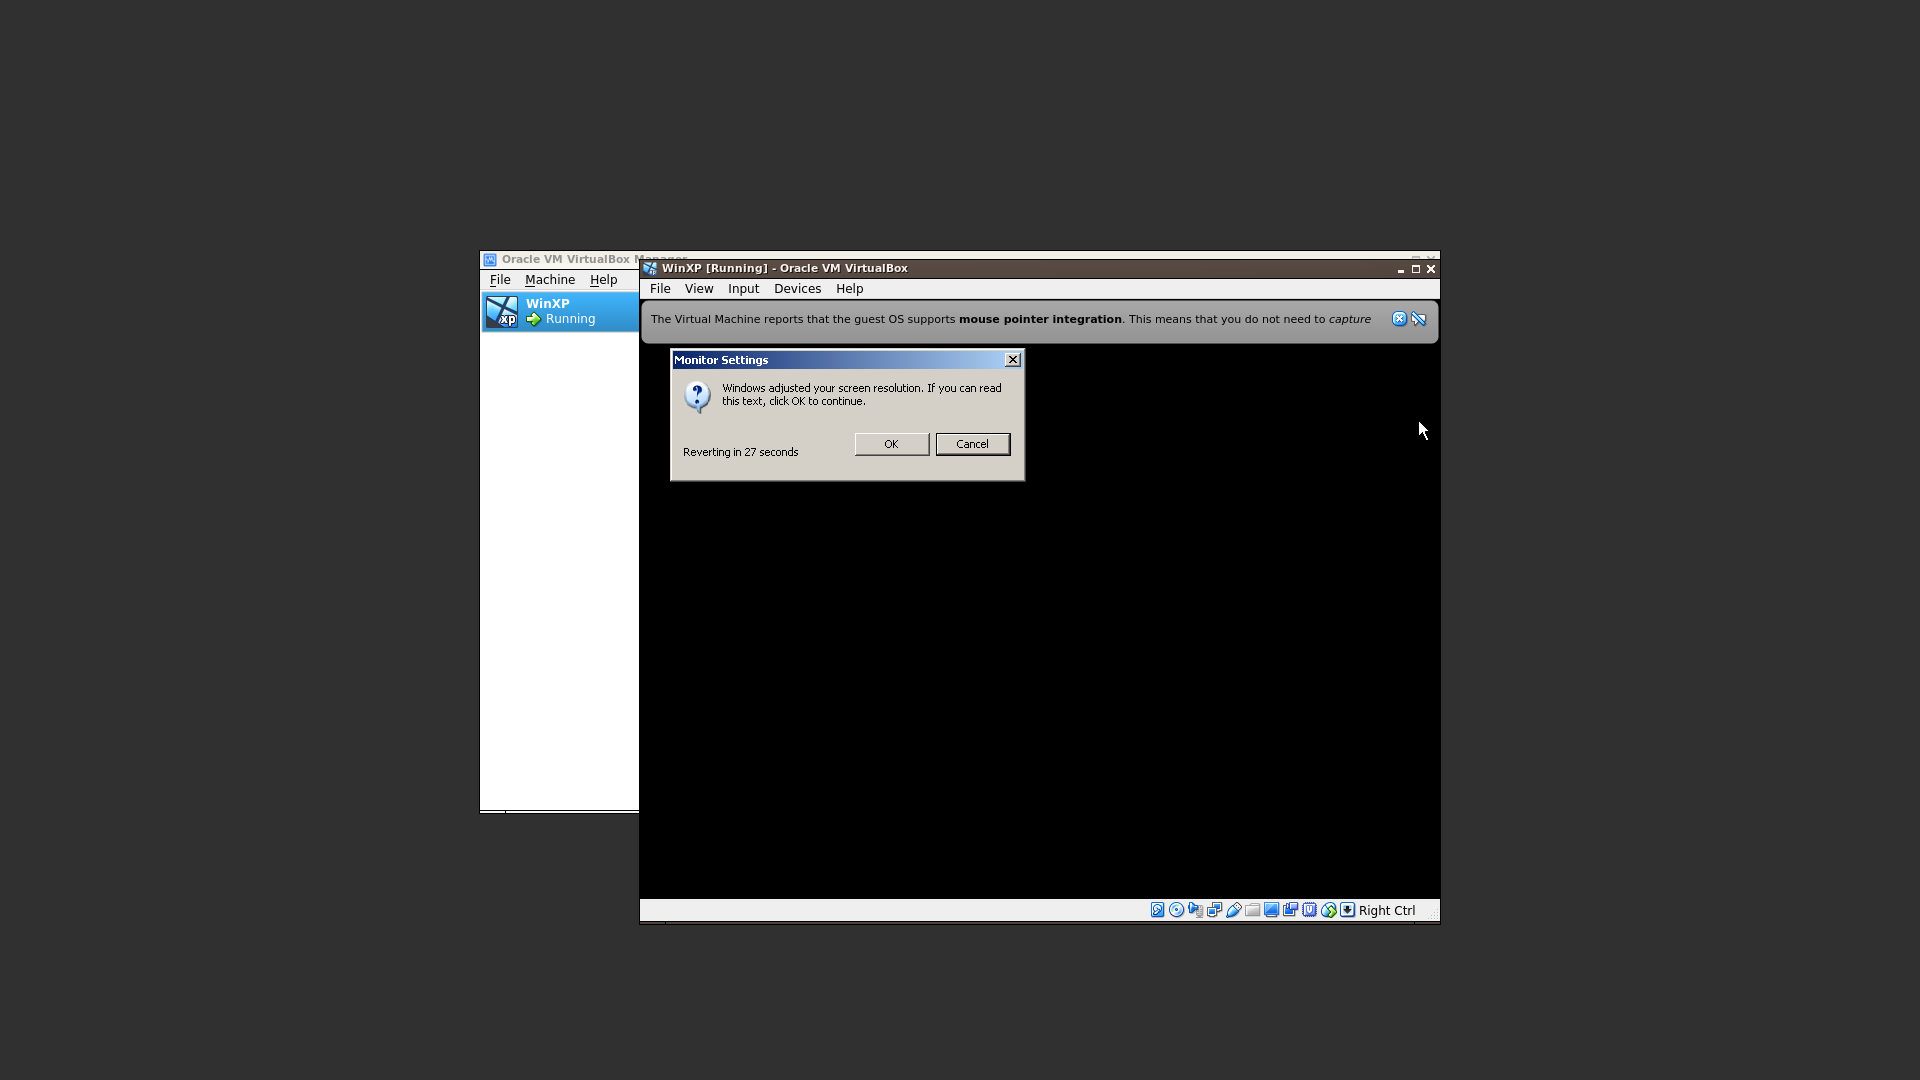
\includegraphics[width=\linewidth]{21.png}
    \caption{Переключилось в новое разрешение}
\end{figure}

\begin{figure}[H]
    \centering
    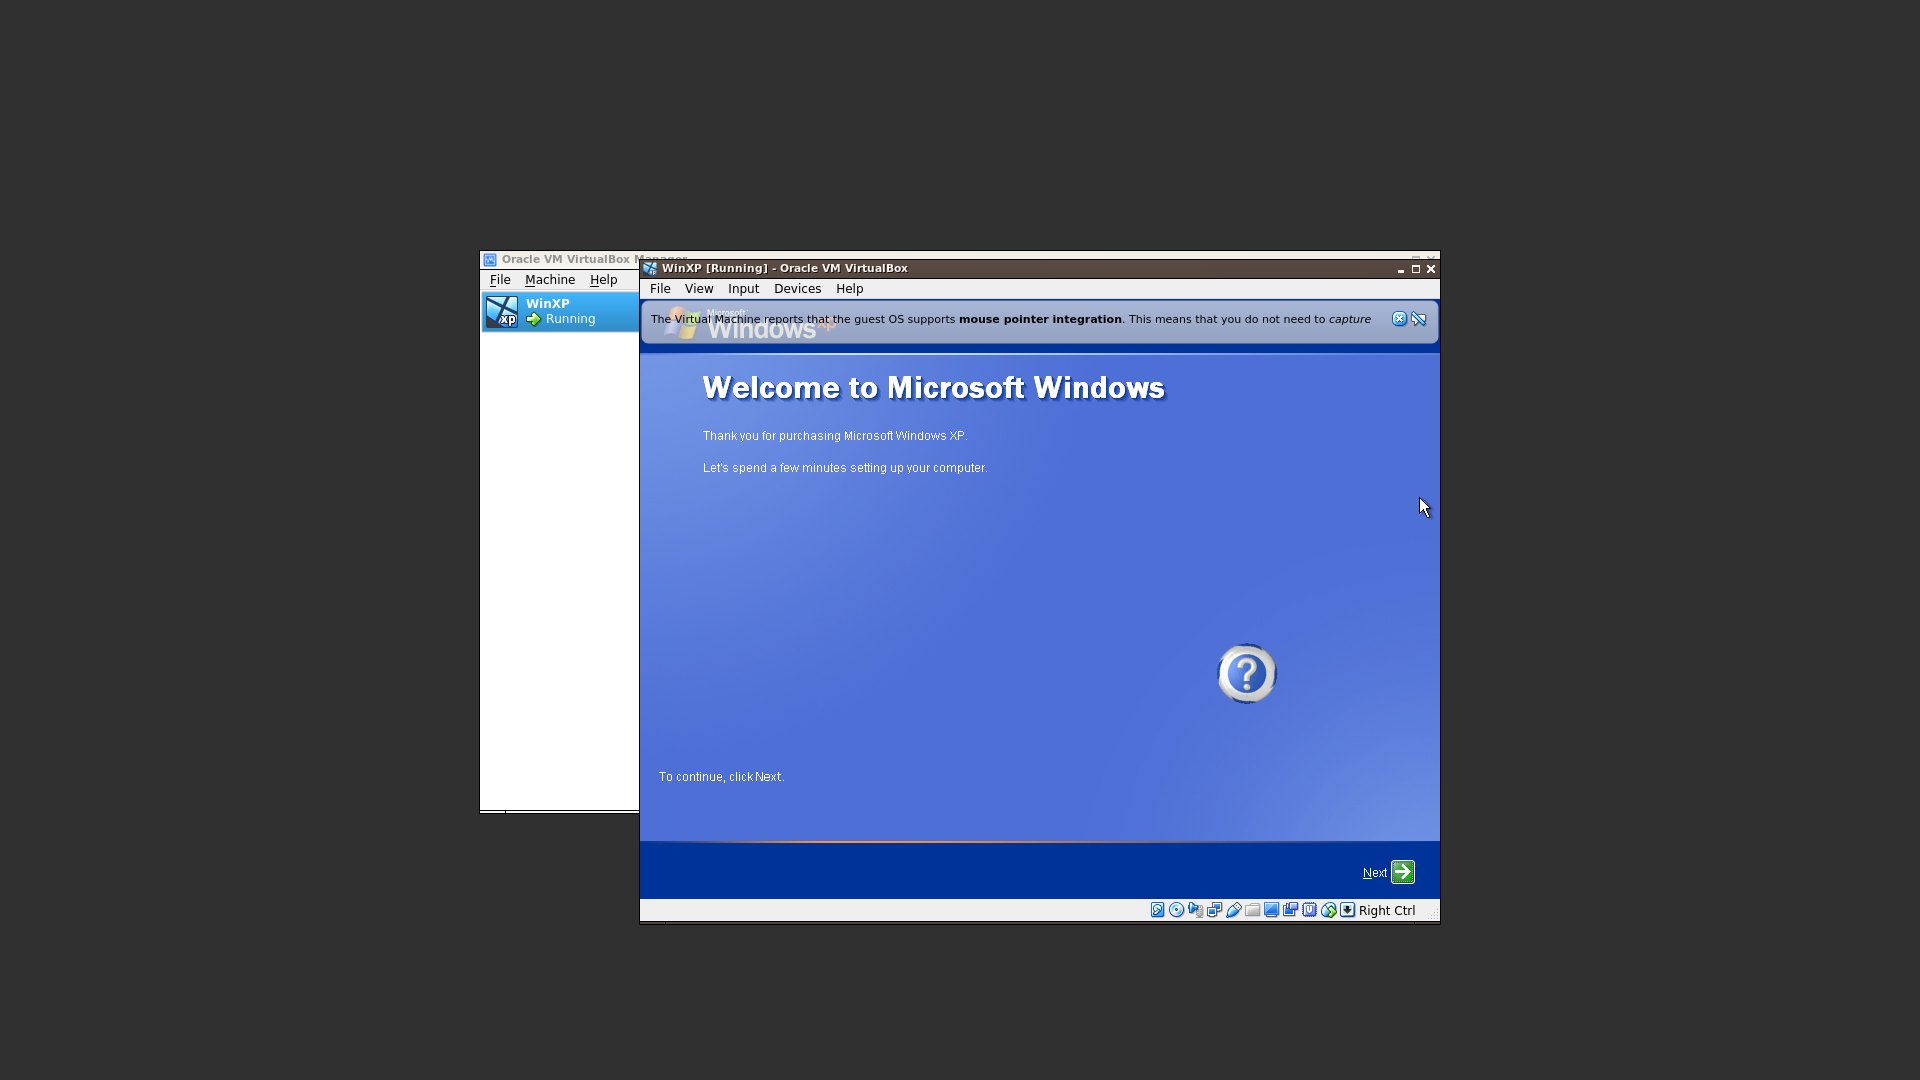
\includegraphics[width=\linewidth]{22.png}
    \caption{Благодарят за приобретение лицензии}
\end{figure}


\begin{figure}[H]
    \centering
    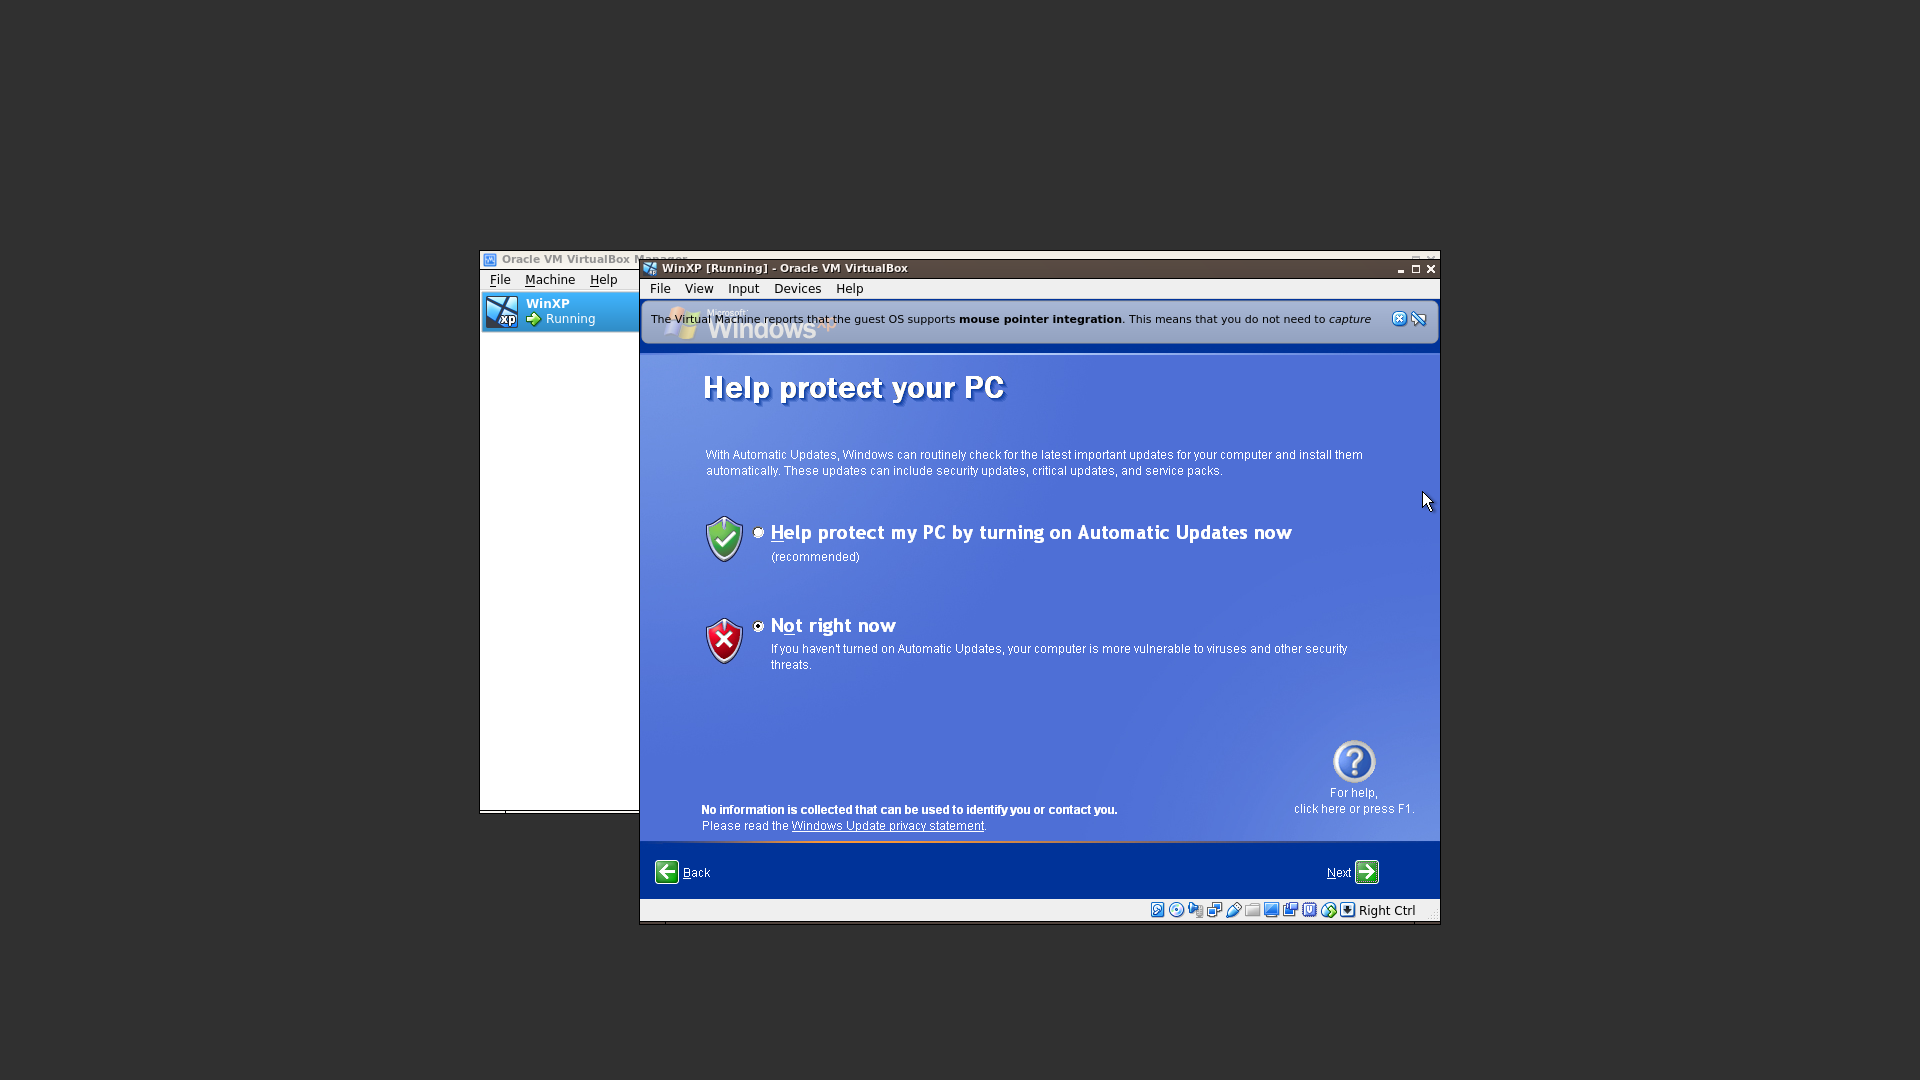
\includegraphics[width=\linewidth]{23.png}
    \caption{Выключаю встроенную защиту}
\end{figure}

\begin{figure}[H]
    \centering
    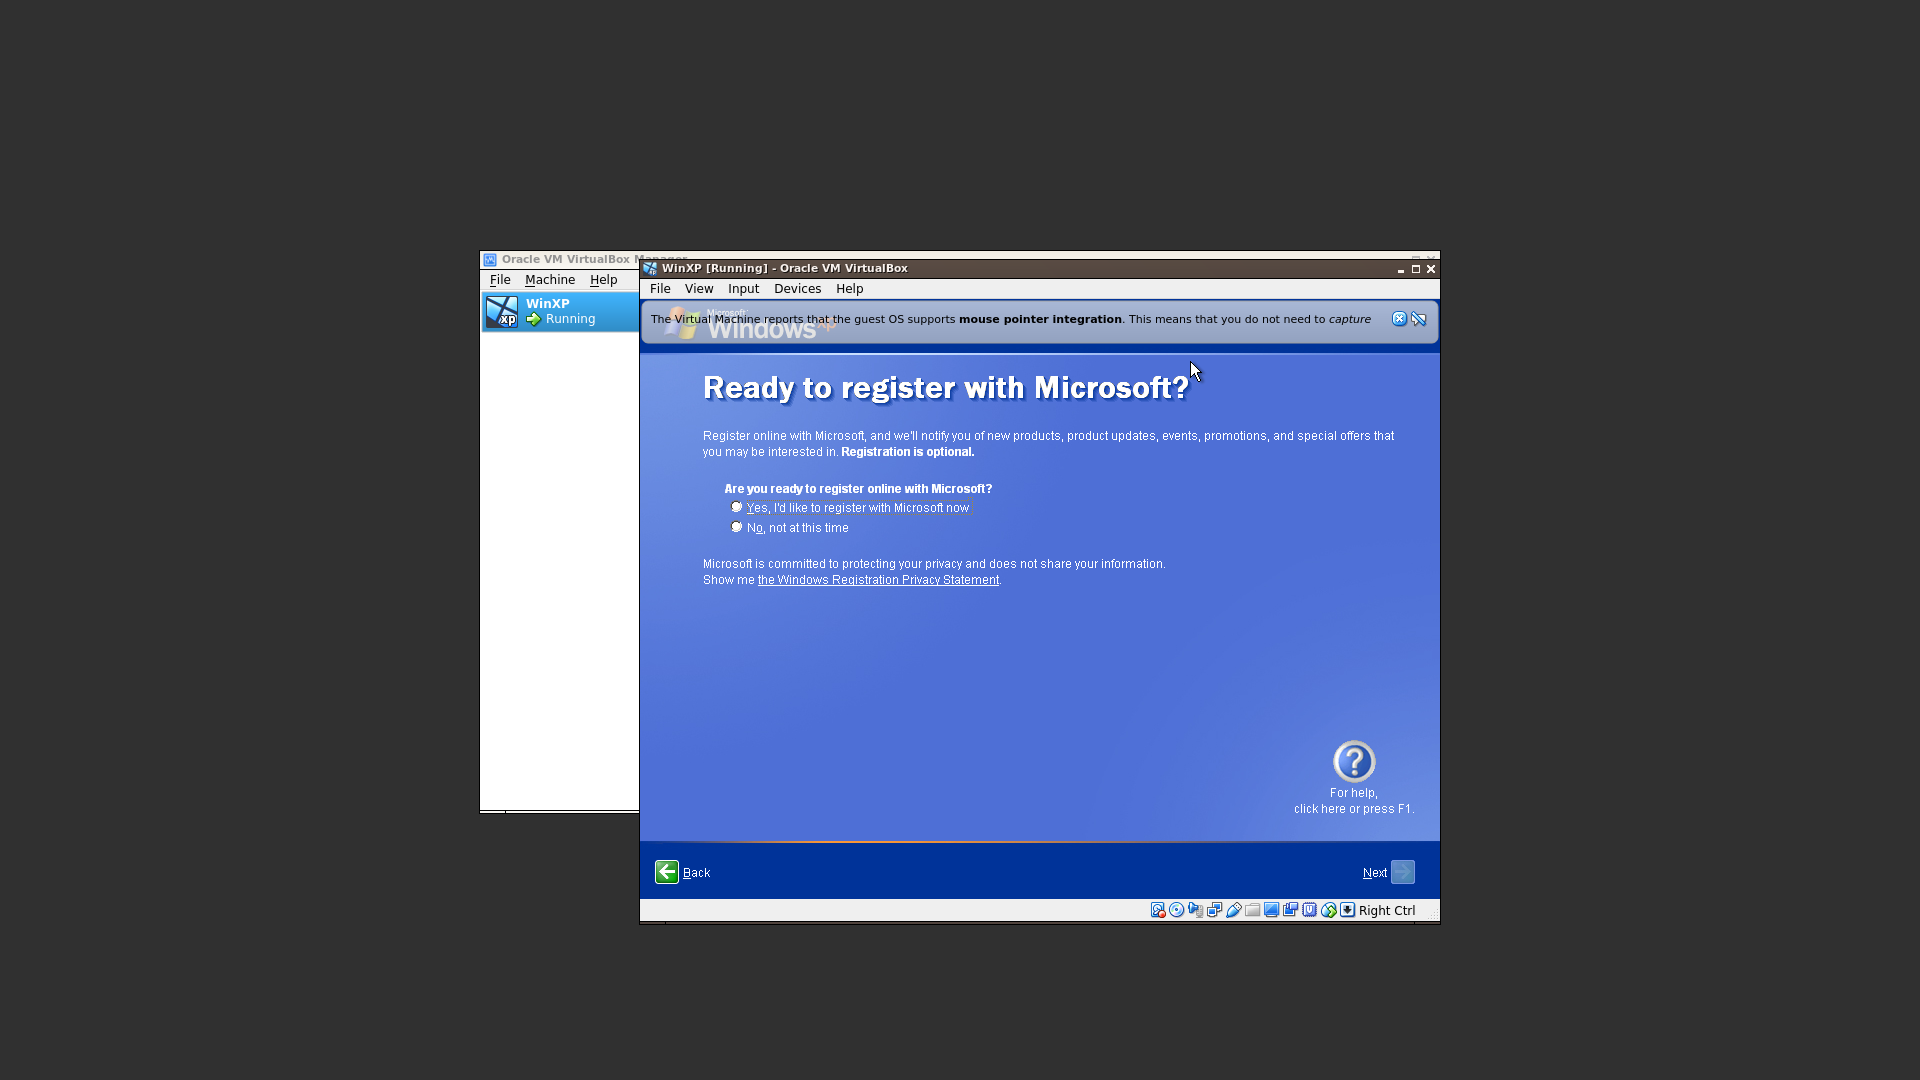
\includegraphics[width=\linewidth]{26.png}
    \caption{Отказываюсь от создания учетной записи}
\end{figure}

\begin{figure}[H]
    \centering
    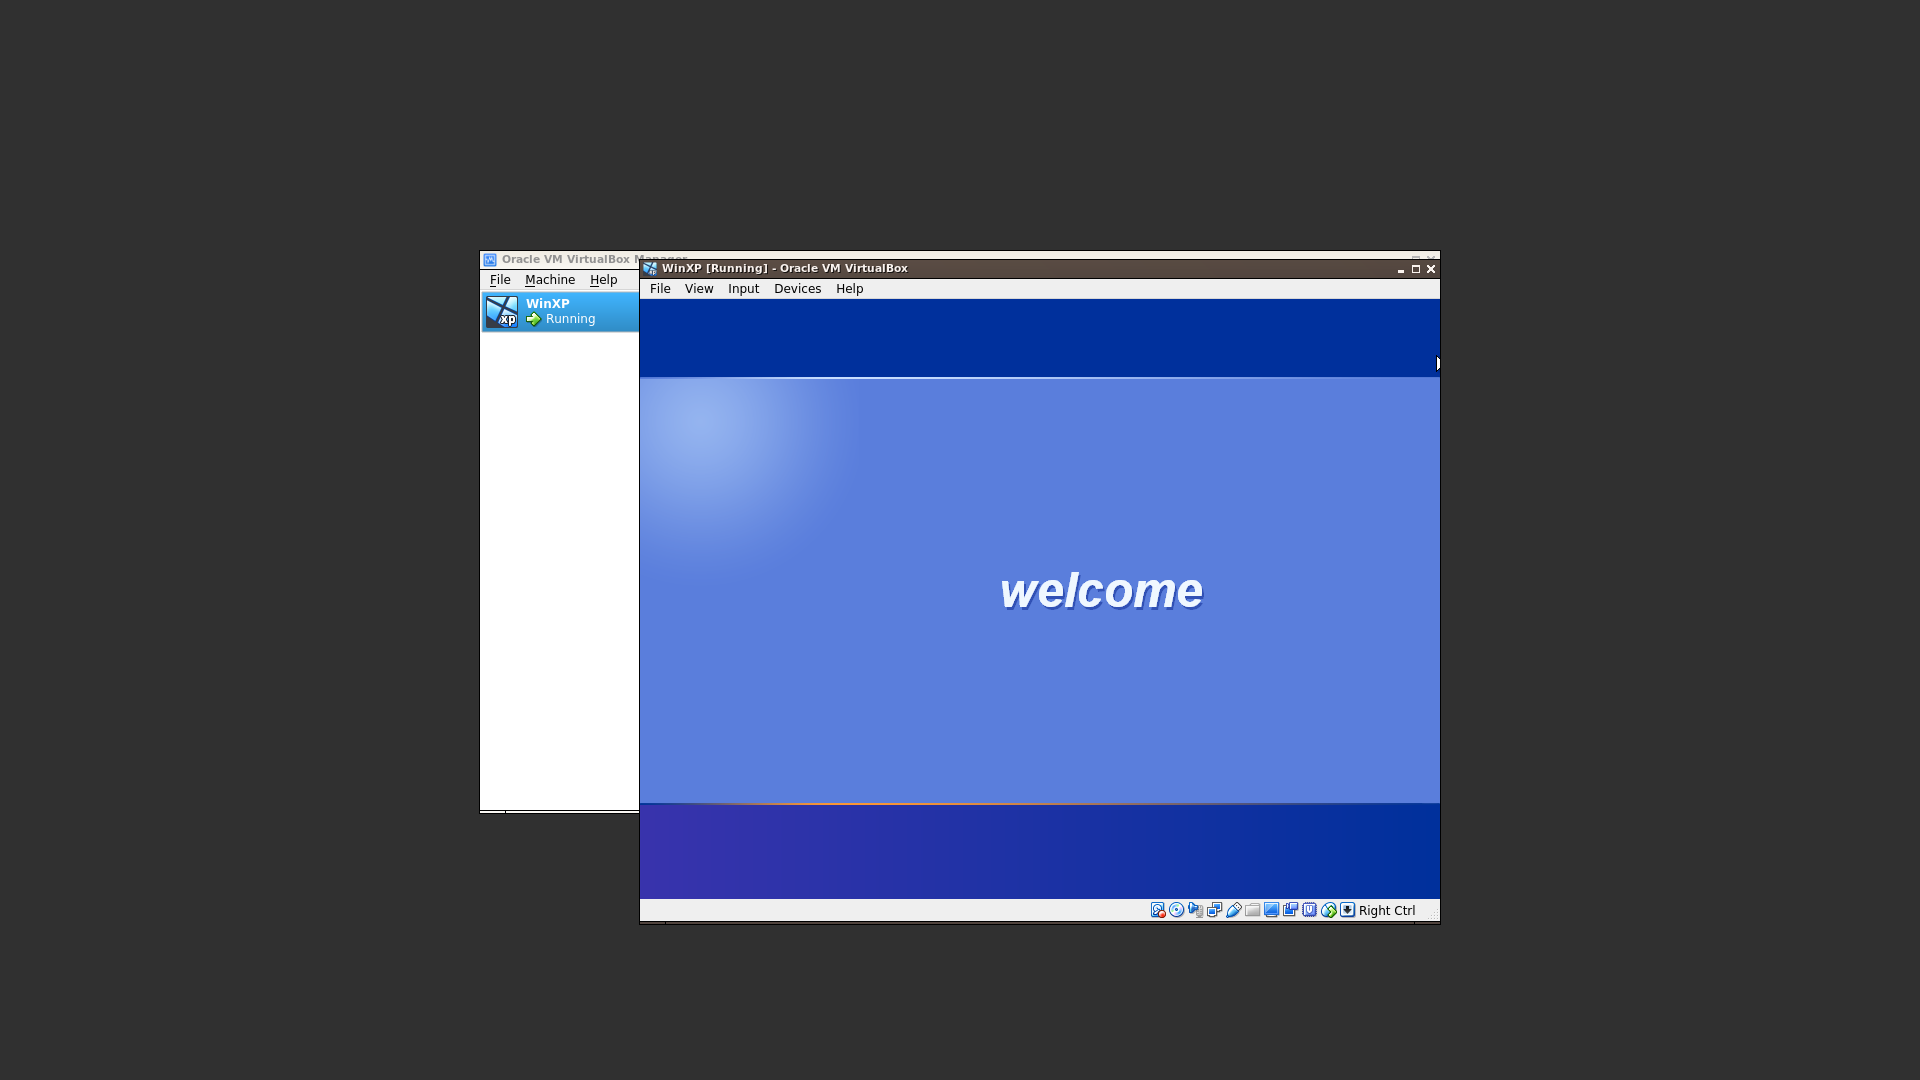
\includegraphics[width=\linewidth]{27.png}
    \caption{Welcome}
\end{figure}

\begin{figure}[H]
    \centering
    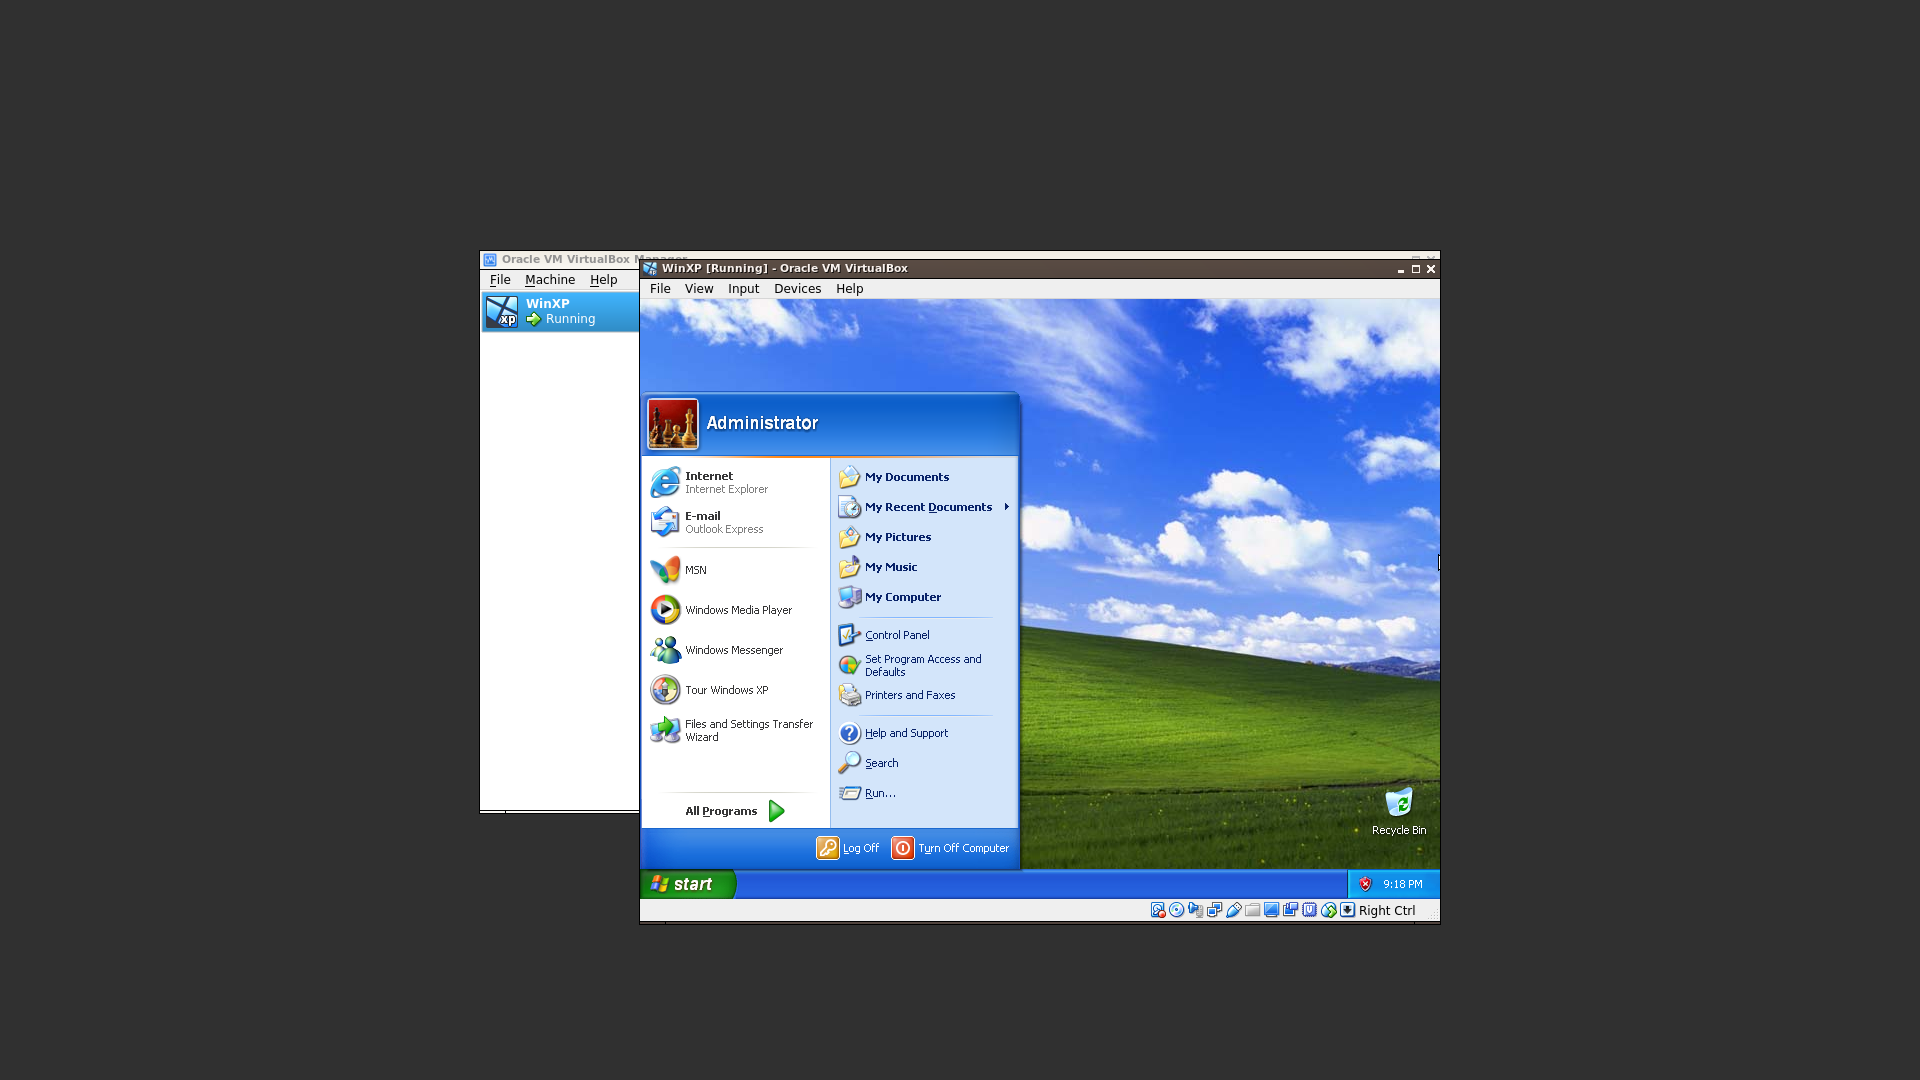
\includegraphics[width=\linewidth]{28.png}
    \caption{Запущена система}
\end{figure}

\begin{figure}[H]
    \centering
    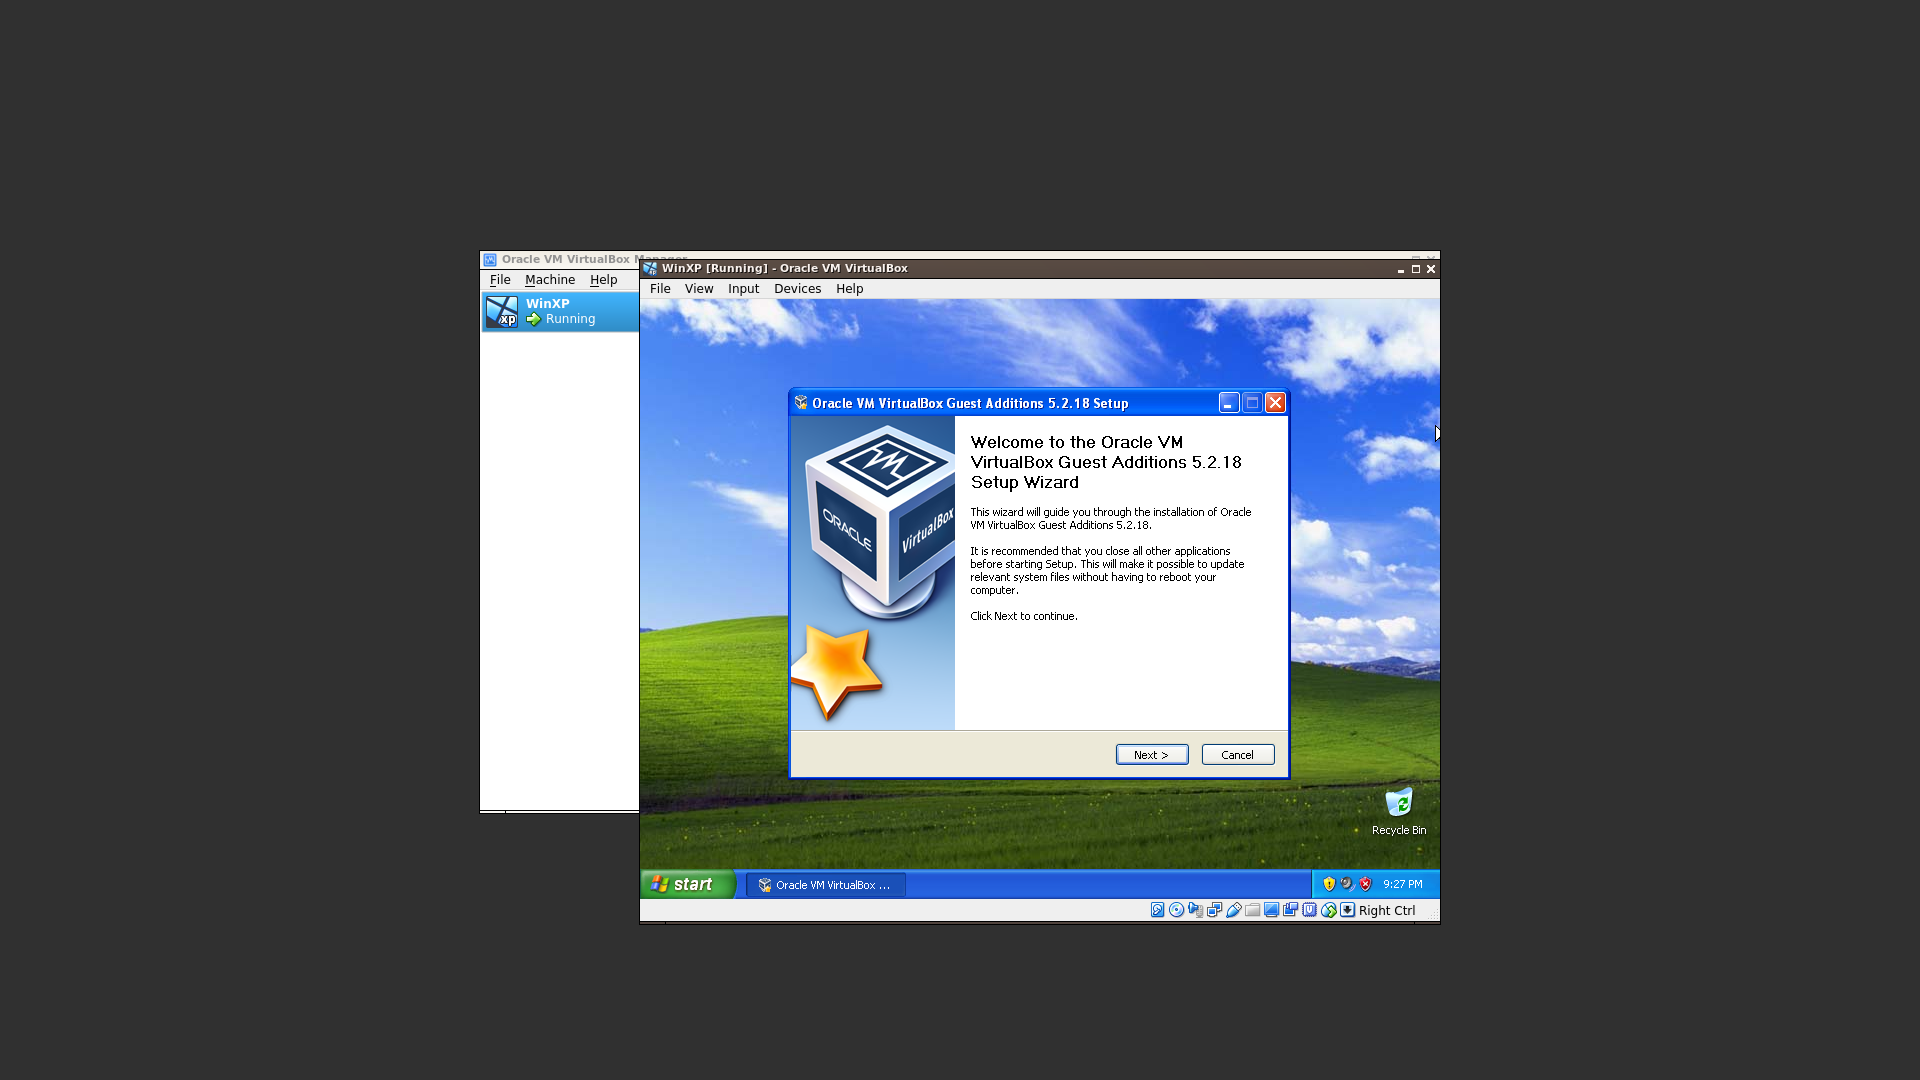
\includegraphics[width=\linewidth]{32.png}
    \caption{Установка по для гостевой системы}
\end{figure}

\begin{figure}[H]
    \centering
    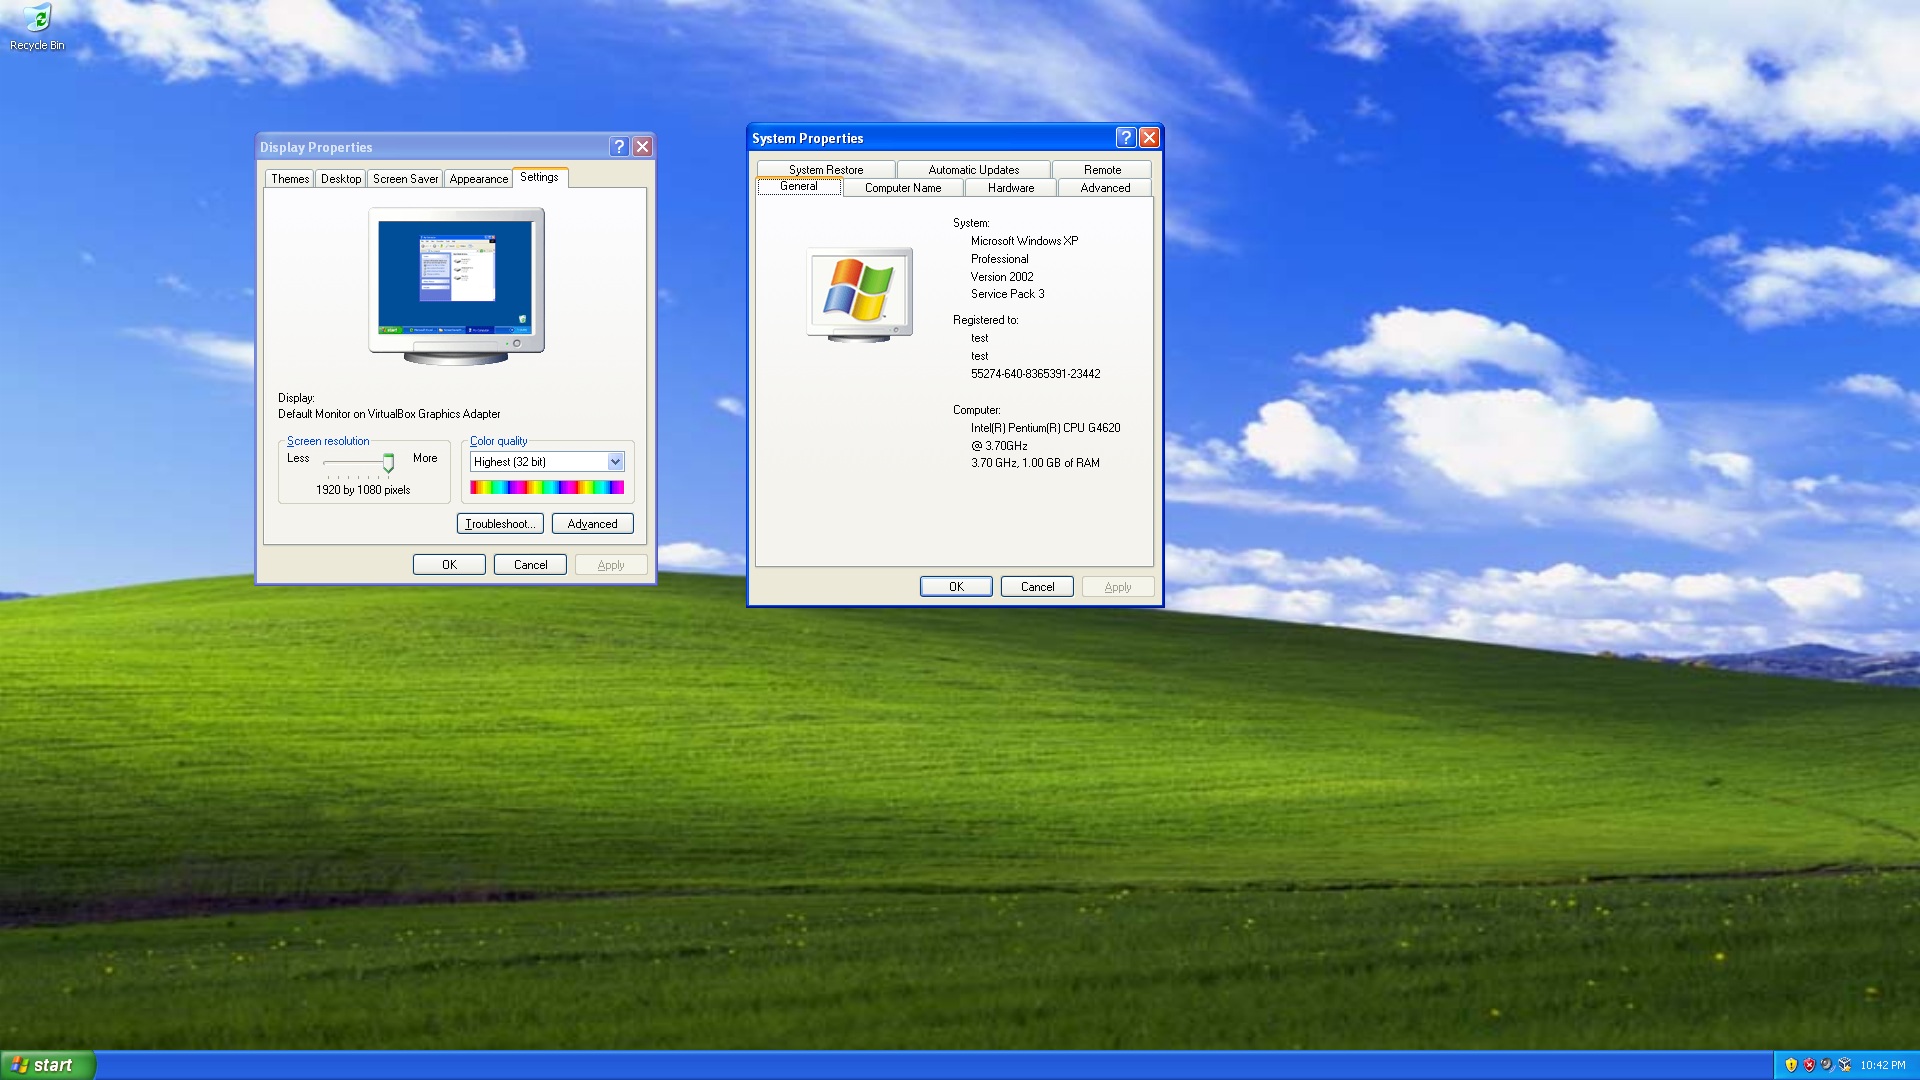
\includegraphics[width=\linewidth]{36.png}
    \caption{ПО для гостевой системы установлено}
\end{figure}


\section{Выводы по работе}

Windows XP установлена на виртуальную машину.

\section{Список использованных источников}

\end{document}
